

\newpage



%----------------------------------------------------------------------------------------


\section[Spatio-temporal Causalities][Causalités Spatio-temporelles]{Spatio-temporal Causalities}{Causalités Spatio-temporelles}

\label{sec:causalityregimes}

%----------------------------------------------------------------------------------------




%----------------------------------------------

\bpar{This section contributes to the understanding of strongly coupled spatio-temporal processes by describing a generic method based on Granger causality. The method is validated by the robust identification of causality regimes and of their phase diagram for an urban morphogenesis model that couples network growth with density. The application to the real case study of Greater Paris transportation projects shows a link between territorial dynamics, more particularly of real estate and socio-economic, and the anticipated network growth. We finally discuss potential extensions to other temporal and spatial scales. Spatial statistics studies on dynamical relations between network and territories are relatively rare. \cite{levinson2008density} does so on London metropolitan area and identifies causalities using lagged variables, but does not disentangle relations in the sense of coupled statistical models that would isolate endogenous effects from coupling effects. study on london with temporal and spatial lag (weird use of spatial statistics). expected conclusions but does not really disentangle ?
In the particular case of relations between network and territories, studies mainly in econometrics have tried to establish causality relationships between variables linked to these two objects. For example, \cite{levinson2008density} explains for the case of London population and connectivity to network variables by these same variables lagged in time, unveiling circular causal effects. \cite{doi10.1068/b39089} uses similar techniques for a region in Italy with historical data on long time, but stays moderate on possible conclusions of systematic effects by recalling the importance of historical events on the estimated relations. \cite{cuthbert2005empirical} proceeds to econometric estimations of reciprocal influence, and concludes that in their Canadian case study at a sub-regional scale, the development of the network induces the development of land-use but not the contrary. Space and time scales influence thus significantly the results of such analysis. \cite{koninghal-00962384} proposes an estimation of relations between the existence of a High Speed Rail connection and economic variables on French Urban Units, and shows a negative effect of the connection itself, after controlling on the endogenous nature of the connection by a selection model, and a significant effect of the characteristics of Urban Units. This work stays limited as it takes neither a time lag larger than one time step nor spatial relations between entities. Finally, still in the same spirit but without explicit inclusion of space, \cite{MANCMANC1073} shows on long time a causality link between infrastructure stock and economic growth on a global panel, but that these effects are moderated locally by under or over-investments.

}{
Cette section contribue à la compréhension des processus spatio-temporels fortement couplés, en proposant une méthode générique basée sur la causalité de Granger. Celle-ci est validée par l'identification robuste de régimes de causalité et de leur diagramme de phase pour un modèle de morphogenèse urbaine couplant croissance du réseau et de la densité. L'application au cas réel de l'Afrique du Sud démontre des liens évolutifs, témoins des évènements historiques entre les dynamiques démographiques territoriales et la croissance du réseau. L'utilisation de statistiques spatiales dur les relations dynamiques entre réseaux et territoires, c'est à dire cherchant à exhiber des relations de causalité, sont relativement rares. Par exemple, \cite{levinson2008density} explique pour Londres les variables de population et de connectivité au réseau par ces mêmes variables décalées dans le temps, démontrant des effets causaux réciproques. \cite{doi:10.1068/b39089} utilise des techniques similaires sur une région d'Italie sur des données historiques sur le temps long, mais modère les conclusions en rappelant l'importance des évènements historiques sur les relations estimées. \cite{cuthbert2005empirical} procède à des estimations économétriques des influences réciproques, et conclut que dans le cas d'étude (au Canada à une échelle sous-régionale) le développement du réseau induit le développement de l'usage du sol, mais pas l'inverse. L'échelle de temps et d'espace devrait logiquement être responsable de cette non-circularité. \cite{koning:hal-00962384} procède à une analyse économétrique de la relation entre existence d'une desserte TGV et variables économiques sur les unités urbaines Françaises, et conclut à un effet propre de la desserte négatif, après contrôle de l'endogénéité de la desserte par un modèle de selection, et un effet significatif des caractéristiques propres des unités urbaines. Cette étude reste limitée car non spatialisée et ne prenant en compte un décalage d'une unité de temps seulement. \cite{MANC:MANC1073} montre sur le temps long un lien de causalité entre stock d'infrastructure et croissance économique sur un panel mondial, mais que ces effets sont atténués localement par des sous ou sur-investissements.
\comment{\cite{carrouet:hal-00980002}}

}




%%%%%%%%%%%%%%%
\subsection[Spatio-temporal Causalities][Causalités Spatio-temporelles]{A method to unveil spatio-temporal causalities}{Une méthode pour identifier des causalités spatio-temporelles}
%%%%%%%%%%%%%%%


\bpar{The study of strongly coupled spatio-temporal processes implies to understand tangled intrications generally highly difficult to isolate. These interactions are the essence of complexity approaches, and are indeed at the origin of the emergent behavior of the system. They make sense as an object of study in itself and a separation of processes appears then contradictory with an integrated view of the system. In the case of territorial systems, the example of interactions between transportation networks and territories is a perfect allegory of this phenomenon: methods developed in the seventies aimed at isolating the ``structuring effects'' of a transportation infrastructure~\cite{bonnafous1974methodologies} have later been unveiled as a political instrument and with a poor empirical support~\cite{offner1993effets}. The issue is still highly relevant today as it raises for example with the construction of new High Speed Rail lines in France~\cite{crozethalshs01094554}. The reality of territorial processus is in fact much more complicated than a simple causal relation between the introduction of a new infrastructure and spillovers on local development, but corresponds indeed to complex \emph{co-evolutive} processes~\cite{bretagnolletel00459720}. On long time scales and large spatial scales, some effects of dynamics reinforcement in system of cities by the insertion within networks have been shown by the application of the Evolutive Urban Theory~\cite{espacegeo2014effets}, showing that the disentangling is sometimes possible through a more global understanding of the system. At an other scale, still for relations between networks and territories, we can point at the relations between mobility practices, urban sprawl et ressource localisation in a metropolitan framework~\cite{cerqueira2017inegalites} that are as much complex. This kind of issue is naturally present in other fields: in Economic Geography, the example of links between innovation, local spillovers of knowledge and aggregation of economic agents is a typical illustration of spatio-temporal economic processes exhibiting circular causalities difficult to disentangle~\cite{audretsch1996r}. Specific methods are introduced, as the use of statistical instruments: \cite{aghion2015innovation} shows that the geographical origin of US Congress members that attribute local subsidies is a powerful instrumental variable to link innovation and income inequalities for higher incomes, what confirms that the significant correlation between the two is indeed a causality of innovation on inequalities.
}
{
L'étude des processus spatio-temporels fortement couplés implique la prise en compte d'intrications entre ceux-ci généralement difficiles à isoler. Essence même des approches par la complexité, ces interactions qui sont à l'origine du comportement émergent d'un système font sens comme objet d'étude en lui-même, et une séparation des processus paraît alors contradictoire avec une vision intégrée du système. Dans le cas des systèmes territoriaux, l'exemple des interactions entre réseaux de transport et territoires est une excellente allégorie de ce phénomène : des méthodes isolant les ``effets structurants'' d'une infrastructure développées dans les années 70~\cite{bonnafous1974methodologies} se sont révélées par la suite de l'instrumentation politique et sans fondement empirique~\cite{offner1993effets}. Le débat est toujours d'actualité puisque la question se pose toujours par exemple pour la construction de lignes à grande vitesse~\cite{crozethalshs01094554}. La réalité des processus territoriaux est en fait bien plus compliqué qu'une simple relation causale entre la mise en place d'une infrastructure et les retombées sur le développement local, mais correspond bien d'une \emph{co-évolution} complexe~\cite{bretagnolletel00459720}. Sur le temps long et à grande échelle, certains effets de renforcement des dynamiques dans les systèmes de villes par l'insertion dans les réseaux, ont été mis en valeur par l'application de la Théorie Evolutive des Villes~\cite{espacegeo2014effets}, montrant que le démêlage est toutefois possible dans certains cas par une compréhension plus globale du système. A une autre échelle, toujours concernant les relations entre réseaux et territoires, on peut citer les liens entre pratiques de mobilité, étalement urbain et localisation des ressources dans un cadre métropolitain~\cite{cerqueira2017inegalites} qui s'avèrent tout autant complexes. Ce type de problématique est bien sûr présent dans d'autres domaines : en Economie Géographique, l'exemple des liens entre innovation, impacts locaux de la connaissance et aggregation des agents économiques est une illustration typiques de processus économiques spatio-temporels présentant des causalités circulaires difficiles à démêler~\cite{audretsch1996r}. Des méthodes spécifiques sont introduites, comme l'utilisation d'instruments statistiques comme par~\cite{aghion2015innovation} dans lequel l'origine géographique des membres du Bureau du Congrès américain attribuant les subventions locales est une bonne variable instrumentale pour lier caractère innovant et inégalités des plus haut salaires, et permet de montrer que la correlation significative entre les deux est en fait une causalité de l'innovation sur les inégalités.
}


\bpar{
Strong coupling in space and time generally implies a notion of causality, that geography has always studied: \cite{loi1985etude} shows that fundamental issues tackled by contemporary theoretical geography (isolation of objects, link between space and causal structures, etc.) were already implicit in Vidal's classical geography. Beside, \cite{claval1985causalite} criticizes the new determinisms having emerged, in particular the one advocated by some scholars of systemic analysis: in its beginning, this approach inherited from cybernetics and thus of a reductionist vision implying a determinism even for a probabilistic formulation. Claval observes that works contemporary to his writings could allow to capture the complexity that characterizes human decisions: the Prigogine School and the Theory of Catastrophes by René Thom. This viewpoint is extremely visionary, since as Pumain recalls in~\cite{pumain2003approche}, the shift from system analysis to self-organisation and complexity has been long and progressive, and these works have played a fundamental role for it. François Durand-Dastès sums up this picture more recently in~\cite{durand2003geographes}, by focusing on the importance of bifurcations and path-dependency in the initial moments of the constitution of a system that he defines as \emph{systemogenesis}. This type of complex dynamics generally implies a co-evolution of system components, that can be understood as circular causalities between processes: the issue of identifying them is thus crucial regarding the notion of causality for contemporary complex geography.
}{
Le couplage fort spatio-temporel implique généralement l'introduction de la notion de causalité, à laquelle la géographie s'est toujours intéressée : \cite{loi1985etude} montre que les questions fondamentales que se pose la géographie théorique récente (isolation des objects, lien entre espace et structures causales, etc.) étaient déjà présentes dans la géographie classique de Vidal. \cite{claval1985causalite} critique d'ailleurs les nouveaux déterminismes ayant émergé, notamment celui proposé par certains tenants de l'analyse systémique : dans ses débuts, cette approche héritait de la cybernétique et donc d'une vision réductionniste impliquant un déterminisme même dans une formulation probabiliste. Claval note que des travaux contemporains à son écriture devraient permettre de capturer la complexité qui fait la particularité des décisions humaines : l'école de Prigogine et la Théorie des Catastrophes de Thom. Ce point de vue est remarquablement visionnaire, puisque comme le rappelle Pumain dans \cite{pumain2003approche}, le glissement de l'analyse des systèmes à l'auto-organisation puis à la complexité a été long et progressif, et ces travaux ont été fondamentaux pour le permettre. François Durand-Dastès résume cette situation plus récemment dans \cite{durand2003geographes}, en appuyant l'importance des bifurcations et de la dépendance au chemin lors des instants initiaux de la constitution du système qu'il désigne par \emph{systèmogenèse}. % note : here we could introduce morphogenesis, form as system structure, linked to circular causalities ; topology and dynamical systems in network propagation (paper Nature Networks). Too far, but keep in mind for further work ?
Ce type de dynamique complexe implique généralement une co-évolution des composantes du système, qu'on peut interpréter comme des causalité circulaires entre processus : la question de pouvoir les identifier est donc cruciale au regard de la notion de causalité pour la géographie complexe contemporaine.
}


\bpar{

The regimes under which identification of causalities are relevant are not obviously known. These will depend of the definitions used, as well as available methods for which we give now a few examples. \cite{liu2011discovering} proposes to detect spatio-temporal relations between perturbations of trafic flows, introducing a particular definition of causality based on correspondance of extreme points. Associated algorithms are however specific and difficult to apply to other kind of systems. The use of spatio-temporal correlations has been shown to have in some cases a strong predictive power for trafic flows~\cite{min2011real}. Also in the field of transportation and land-use, \cite{xie2009streetcars} applies a Granger causality analysis, that can be interpreted as lagged correlation, to show for a case study that network growth inducts urban development and is itself driven by externalities such as mobility habits. Neuroscience has developed numerous methods answering similar issues. \cite{luo2013spatio} defines a generalized Granger causality that takes into account non-stationarity and applies to abstracts regions produced by functional imaging. This kind of method is also developed in Computer Vision, as illustrated by \cite{ke2007spatio} that exploits spatio-temporal correlations of forms and flows between successive images to classify and recognize actions. Applications can be quite concrete such as compression of video files by extrapolation of motion vectors~\cite{chalidabhongse1997fast}. In all these cases, the study of spatio-temporal correlations meets the weak notions of causality described above. This contribution aims to explore the possibility of a similar methods for spatio-temporal data exhibiting a priori complex circular causalities, and thus to realize the difficult exercise to couple a certain level of simplicity with a grasping of complexity. We introduce therefore a method to analyse spatio-temporal correlations, similar to a Granger causality estimated in space and time. The robustness of the method is demonstrated in a systematic way by the application to a complex model of simulation of urban morphogenesis, what leads to the unveiling of distinct causality regimes in the phase space of the model. We also include the application to an empirical case study, what positions this work at the interface between knowledge domains of methodology, modeling and empirical within the epistemological framework introduced by~\cite{2017arXiv170609244R}.
}{
Les régimes sous lesquels des identifications de causalité sont cohérentes ne sont pas identifiés de manière évidente. Ceux-ci dépendront des définition utilisées, de la même manière que les méthodes à disposition pour lesquelles nous pouvons donner quelques illustrations. \cite{liu2011discovering} propose la detection de relations spatio-temporelles entre perturbations des flots de trafic, introduisant une définition particulière de la causalité basé sur une correspondance de points extrêmes. Les algorithmes associés sont toutefois spécifiques et difficilement applicables à des types de systèmes différents. L'utilisation des correlations spatio-temporelles a été démontrée comme ayant dans certains cas un fort pouvoir prédictif pour les flots de traffic~\cite{min2011real}. Egalement dans le domaine des transports et de l'usage du sol, \cite{xie2009streetcars} applique une analyse par causalité de Granger, qu'on pourra interpréter comme une corrélation retardée, pour montrer dans un cas particulier que la croissance du réseau induit le développement urbain et est elle-même tirée par des externalités comme les habitudes de mobilité. Les neurosciences ont développé de nombreuses méthodes répondant à des problématiques similaires. \cite{luo2013spatio} définit une causalité de Granger généralisée prenant en compte la non-stationnarité et s'appliquant à des régions abstraites issues d'imagerie fonctionnelle. Ce genre de méthode est également développée en Vision par Ordinateur, comme l'illustre \cite{ke2007spatio} qui exploite les correlations spatio-temporelles de formes et de flux dans des successions d'images pour classifier et reconnaître des actions. Les applications peuvent être très concrète comme la compression de fichier videos par extrapolation des vecteurs de mouvement~\cite{chalidabhongse1997fast}. Dans l'ensemble de ces cas, l'étude des correlations spatio-temporelles rejoint les notions faibles de causalité vues précédemment. Cette contribution cherche à explorer la possibilité d'une méthode analogue pour des données spatio-temporelles présentant a priori des causalités circulaires complexes, et donc de tenter l'exercice d'équilibriste de concilier un certain niveau de simplicité et de caractère opérationnel à une prise en compte de la complexité. Nous introduisons ainsi une méthode d'analyse des correlations spatio-temporelles similaire à une causalité de Granger estimée dans le temps et l'espace, dont la robustesse est démontrée systématiquement par l'application à un modèle de simulation complexe de morphogenèse urbaine et par l'isolation de régimes de causalités distincts dans l'espace des phases du modèle. Notre contribution inclut également l'application à un cas d'étude empirique, ce qui la positionne à l'interface des domaines de la méthodologie, de la modélisation et de l'empirique.
}


\bpar{
The rest of this section is organized as follows: the generic framework of the method is described in the next section. We then apply it to a synthetic dataset to partially validate it and test its potentialities, what allows us to apply it then to the real case study of Grand Paris transportation network. We finally discuss to proximity with existing methods and possible developments.
}{
La suite de cette section est organisée de la façon suivante : le cadre générique de la méthode proposée est décrit. Nous l'appliquons ensuite à un jeu de données synthétiques afin de la valider partiellement et de tester ses potentialité, ce qui permet de l'appliquer ensuite au système urbain Sud-Africain sur le temps long. Nous discutons finalement la proximité avec d'autres méthodes existantes et des développements possibles.
}



%%%%%%%%%%%%%%%
\subsubsection{Method}{Méthode}
%%%%%%%%%%%%%%%


\bpar{
We formalize here the method in a generic way, based in a weak formulation of Granger causality, to try to identify causal relations in spatial systems. Let $X_j(\vec{x},t)$ spatio-temporal unidimensional random processes, which realizations occur in space and time. We give a set of fundamental spatial units  $(u_i)$ that can be for example raster cells or any paving of the geographical space. We assume the existence of functions $\Phi_{i,j}$ allowing to make the correspondance between the realization of each components and spatial units, possibly through a first spatial aggregation or by a more elaborated process driven by a network for example. A realization of a system is given by a set of trajectories for each process $x_{i,j,t}$, and we write a set of realizations $x^{(k)}_{i,j,t}$ (accessible by stochastic repetitions in the case of a model of simulation for example, or by assumption of comparability of territorial sub-systems in real cases). We assume to have a correlation estimator $\hat{\rho}$ applying in time, space and repetitions, i.e. $\hat{\rho}\left[X,Y\right] = \hat{\mathbb{E}}_{i,t,k}\left[XY\right] - \hat{\mathbb{E}}_{i,t,k}\left[X\right]\hat{\mathbb{E}}_{i,t,k}\left[Y\right]$. It is important to note here the hypothesis of spatial and temporal stationarity, that can however easily be relaxed in the case of local stationarity. Furthermore, spatial auto-correlation is not explicitly included, but is taken into account either by the initial spatial aggregation is the characteristic scale of units is larger than the one of neighborhood effects, either by an adequate spatial estimator (weighted spatial statistics of type \emph{GWR}~\cite{brunsdon1998geographically} for example). It allows us to define the lagged correlation by 
}{
Nous formalisons ici de manière générique la méthode, basée sur un test similaire à la causalité de Granger\comment[FL]{c'est la meme chose que gwr}[(JR) ? (ou meme chose pour le besoin d'explicitation ?]\footnote{Se référer au chapitre préliminaire pour la definition mathématique utilisée.}, pour tenter d'identifier des relations causales dans des systèmes spatiaux. Soit $X_j(\vec{x},t)$ des processus aléatoires spatiaux unidimensionnels, se réalisant dans le temps et l'espace. On se donne un ensemble d'unités spatiales fondamentales $(u_i)$ qui peuvent être par exemple les cellules d'un raster ou un pavage quelconque de l'espace géographique. On suppose l'existence de fonctions $\Phi_{i,j}$ permettant de faire correspondre les réalisations de chaque composante aux unités spatiales, possiblement par une première agrégation locale. Une réalisation d'un système est donnée par un ensembles de trajectoires pour chaque processus $x_{i,j,t}$, et on pourra noter un ensemble de réalisations $x^{(k)}_{i,j,t}$ (accessibles dans le cas d'un modèle de simulation par exemple, ou par hypothèse de comparabilité de sous-systèmes territoriaux dans des cas réels). On suppose disposer d'un estimateur de correlation $\hat{\rho}$ s'exerçant dans le temps, l'espace et les répétitions, i.e. $\hat{\rho}\left[X,Y\right] = \hat{\mathbb{E}}_{i,t,k}\left[XY\right] - \hat{\mathbb{E}}_{i,t,k}\left[X\right]\hat{\mathbb{E}}_{i,t,k}\left[Y\right]$. Il est important de noter ici l'hypothèse de stationnarité spatiale et temporelle, qui peut toutefois aisément se relâcher dans le cas d'une stationnarité locale. D'autre part, l'autocorrelation spatiale n'est pas explicitement incluse, mais est prise en compte soit par l'agrégation initiale si l'échelle caractéristique des unités est plus grande que celle des effets de voisinage, soit par un estimateur spatial adéquat (statistiques spatiales pondérées de type \emph{GWR}\footnote{voir également le chapitre de definition}~\cite{brunsdon1998geographically} par exemple). Cela nous permet de définir la correlation retardée par
}

\begin{equation}
\rho_{\tau}\left[X_{j_1},X_{j_2}\right] = \hat{\rho}\left[x^{(k)}_{i,j_1,t - \tau},x^{(k)}_{i,j_2,t}\right]
\end{equation}

\bpar{
The lagged correlation is not symmetric, but we have directly $\rho_{\tau}\left[X_{j_1},X_{j_2}\right] = \rho_{-\tau}\left[X_{j_2},X_{j_1}\right]$. This measure is applied in a simple way: if $\textrm{argmax}_{\tau} \rho_{\tau}\left[X_{j_1},X_{j_2}\right]$ or $\textrm{argmin}_{\tau} \rho_{\tau}\left[X_{j_1},X_{j_2}\right]$ are ``clearly defined'' (both could be simultaneously), their sign will give the sense of causality between components $j_1$ and $j_2$ and their absolute value the propagation lag. The criteria for significance will depend on the case of application and of the estimator used, but can for example include the significance of the statistical test (Fisher test in the case of a Pearson estimator), the position of extremities of a confidence interval of a given level, or even an exogenous threshold $\theta$ on $\left|\rho_{\tau}\right|$ to ensure a certain level of correlation.
}{
La corrélation retardée n'est pas directement symétrique, mais on a de manière évidente $\rho_{\tau}\left[X_{j_1},X_{j_2}\right] = \rho_{-\tau}\left[X_{j_2},X_{j_1}\right]$. On applique alors cette mesure de manière simple : si $\textrm{argmax}_{\tau} \rho_{\tau}\left[X_{j_1},X_{j_2}\right]$ ou $\textrm{argmin}_{\tau} \rho_{\tau}\left[X_{j_1},X_{j_2}\right]$ sont ``clairement définis'' (les deux pouvant l'être simultanément), leur signe donnera alors le sens de la causalité entre les composantes $j_1$ et $j_2$ et leur valeur absolue le retard de propagation. Les critères de significativité dépendront du cas d'application et de l'estimateur utilisé, mais peuvent par exemple inclure la significativité du test statistique (test de Fisher dans le cas d'un estimateur de Pearson), la position des bornes d'un intervalle de confiance à un niveau donné, ou même un seuil exogène $\theta$ sur $\left|\rho_{\tau}\right|$ pour forcer un certain degré de correlation. 
}




%%%%%%%%%%%%%%%
\subsection{Synthetic data}{Données Synthétiques}



%%%%%%%%%%%%%%%
\begin{figure}%[h]
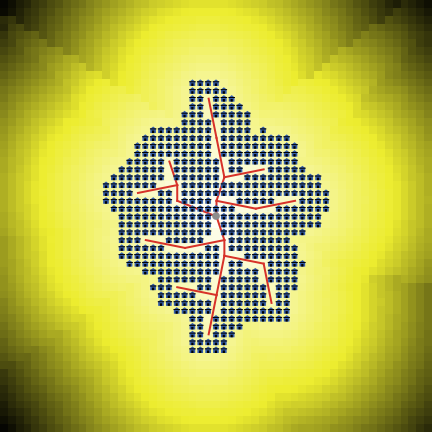
\includegraphics[width=0.32\linewidth]{Figures/CausalityRegimes/ex_60_wdens0_wroad1_wcenter1_seed272727}
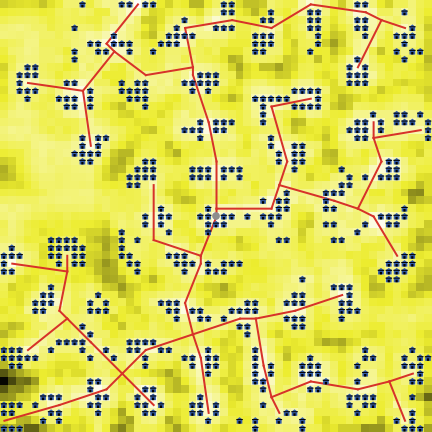
\includegraphics[width=0.32\linewidth]{Figures/CausalityRegimes/ex_60_wdens1_wroad1_wcenter0_seed272727}
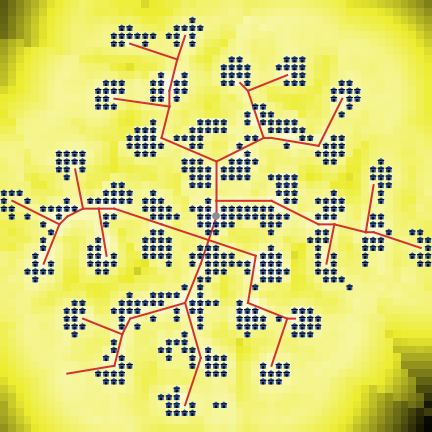
\includegraphics[width=0.32\linewidth]{Figures/CausalityRegimes/ex_60_wdens1_wroad1_wcenter1_seed272727}\\\vspace{0.2cm}
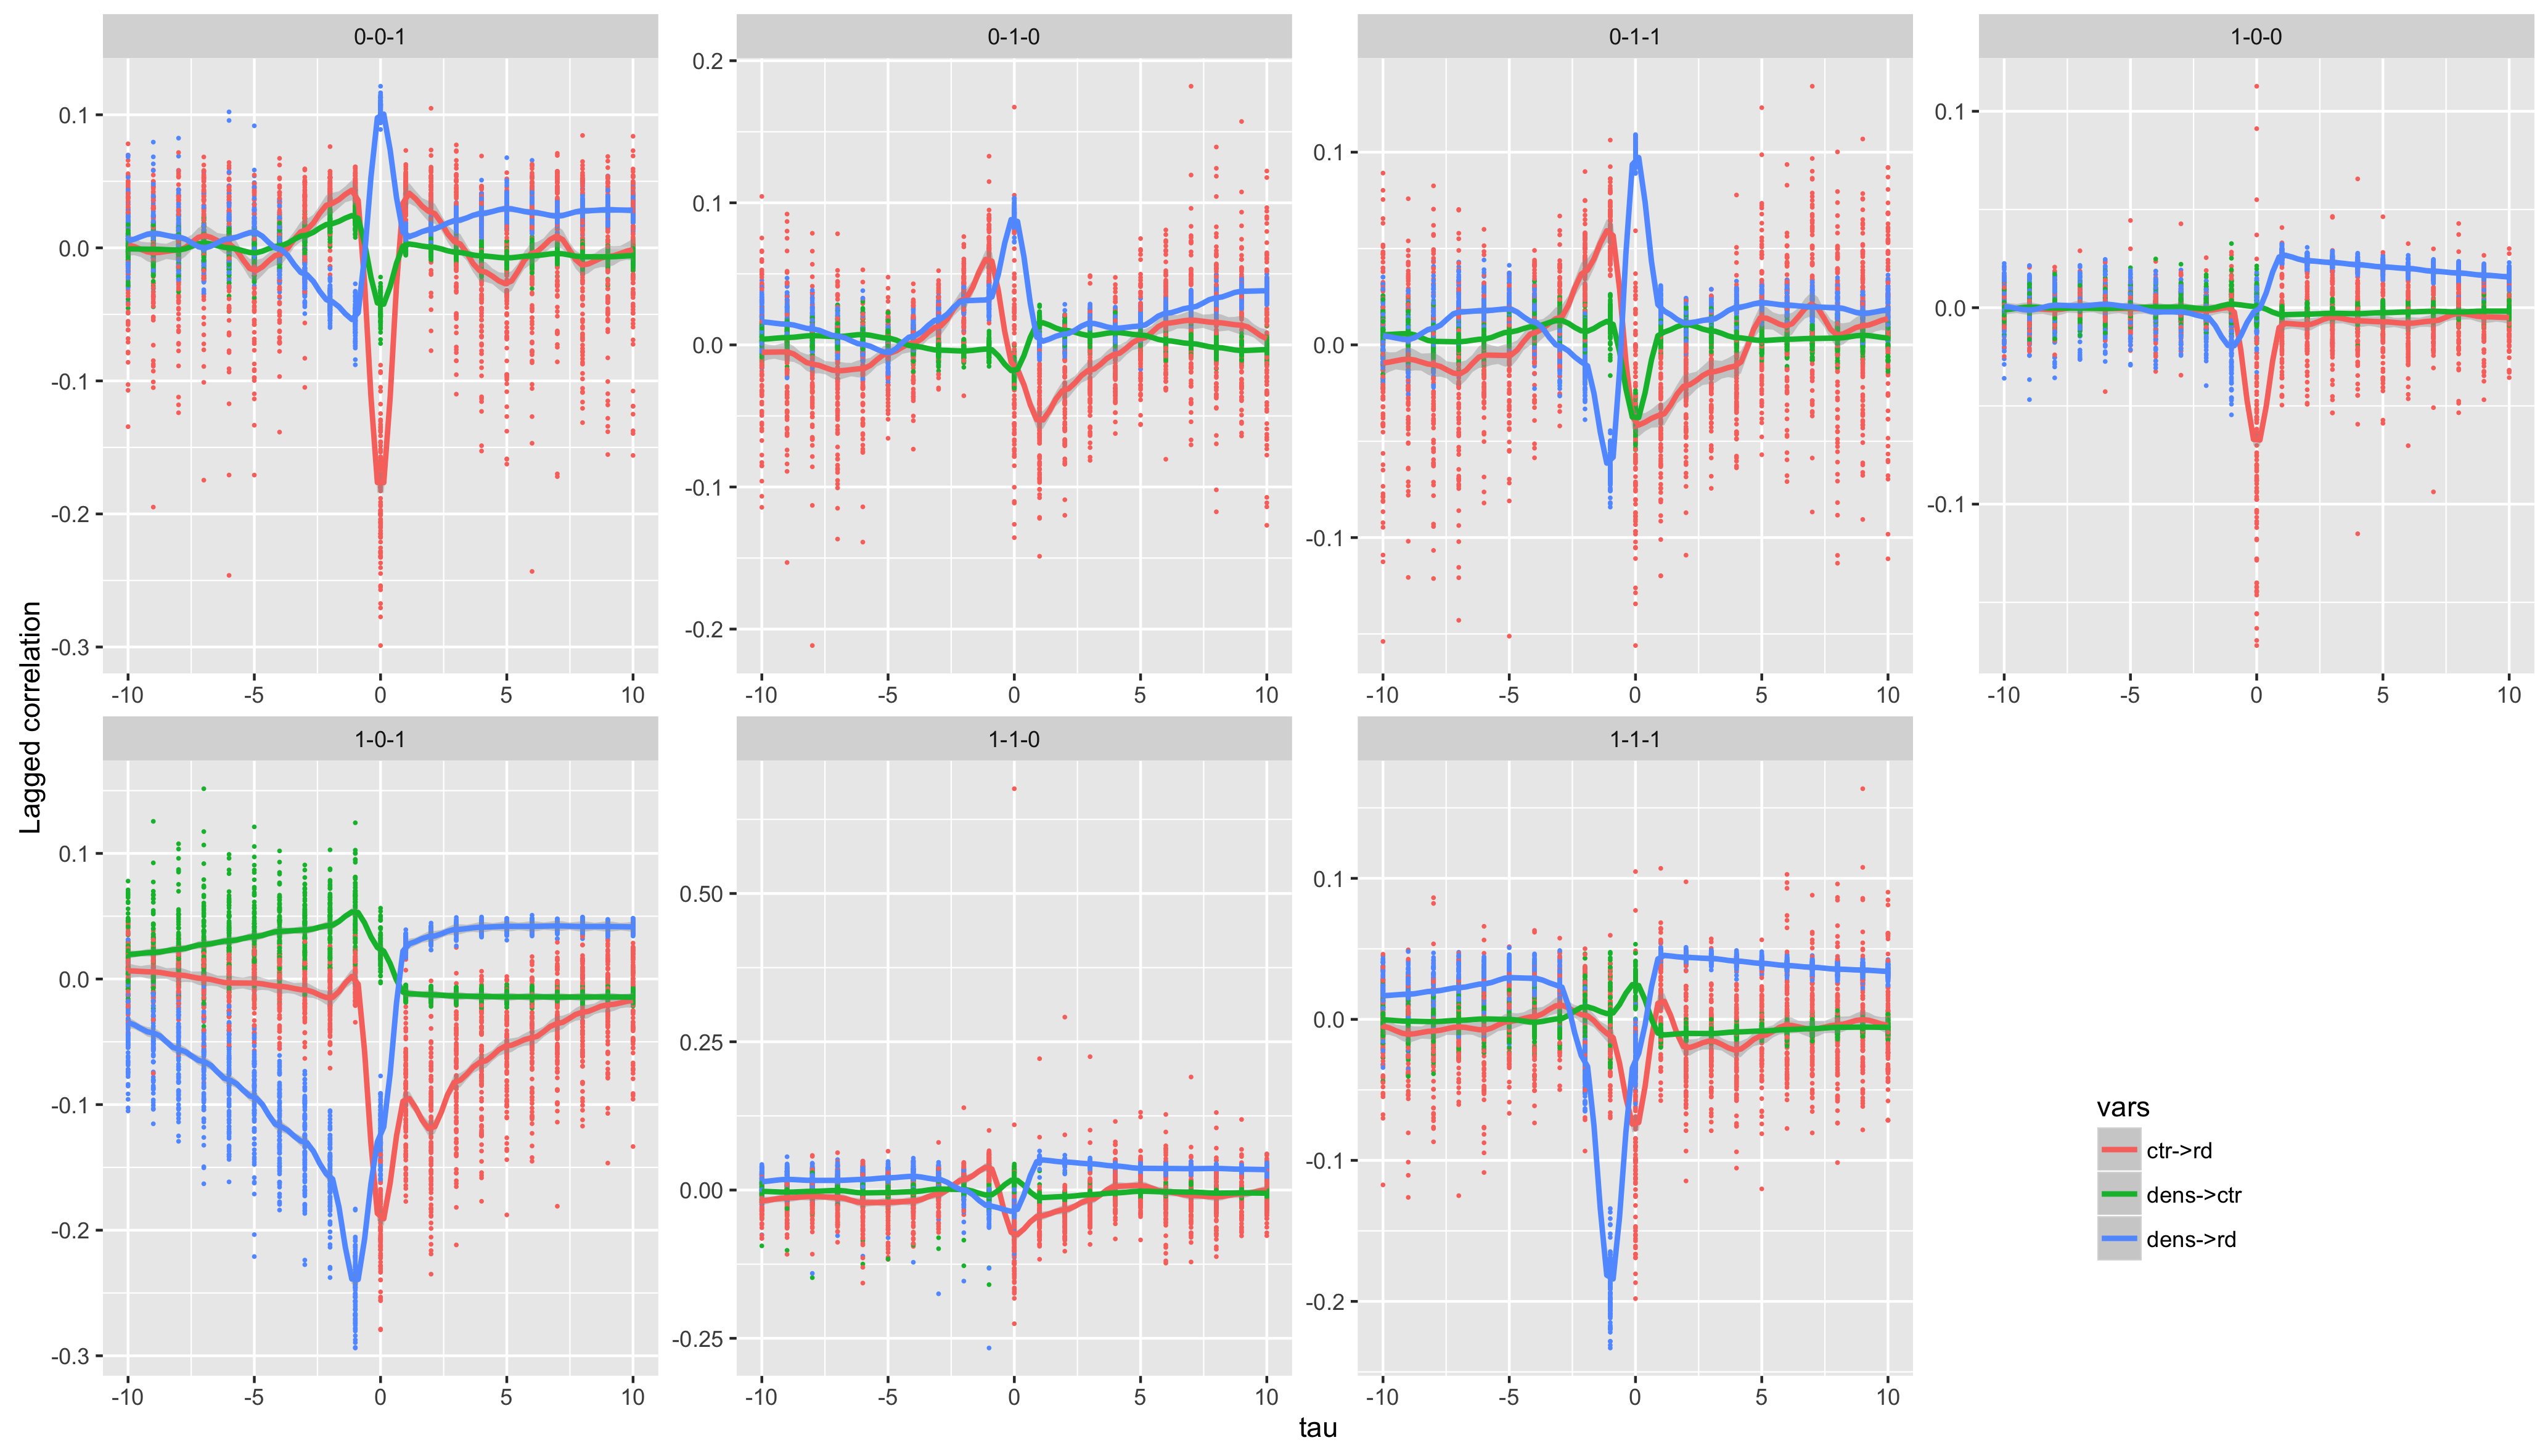
\includegraphics[width=\linewidth]{Figures/CausalityRegimes/laggedcorrs_facetextreme}
\caption[Correlation in the RBD model][Correlations dans le modèle RDB]{\textbf{Correlations in the RBD model.} \textbf{(First row)} Example of different final configurations, obtained with $(w_{d},w_{c},w_{r})$ being respectively $(0,1,1)$,$(1,0,1)$, and $(1,1,1)$. \textbf{(Second row)} Lagged correlations, for each combination of parameters in $\{0,1\}$, as a function of the lag $\tau$. The different colors correspond to each couple of variables: distance to the center (\texttt{ctr}), density (\texttt{dens}) and distance to the network (\texttt{rd}). The dots show the extent on all the repetitions of the model (estimators on $i$ and $t$ only).\label{fig:causalityregimes:exrdb}}{\textbf{Correlations dans le modèle RDB} \textbf{(Première ligne)} Exemples de configurations finales variées, obtenues avec $(w_{d},w_{c},w_{r})$ valant respectivement $(0,1,1)$,$(1,0,1)$, et $(1,1,1)$. \textbf{(Deuxième ligne)} Corrélations retardées, pour chaque combinaison des paramètres, en fonction du retard $\tau$. Les différentes couleurs correspondent à chaque couple de variables : distance au centre (\texttt{ctr}), densité (\texttt{dens}) et distance au réseau (\texttt{rd}). Les points montrent l'étendue sur l'ensemble des répétitions du modèle (estimateurs sur $i$ et $t$).\label{fig:causalityregimes:exrdb}\comment[FL]{que signifient les lignes brisees ? comment sont-elles obtenues ?}}
\end{figure}
%%%%%%%%%%%%%%%



%%%%%%%%%%%%%%%
\begin{figure}%[h]
\centering
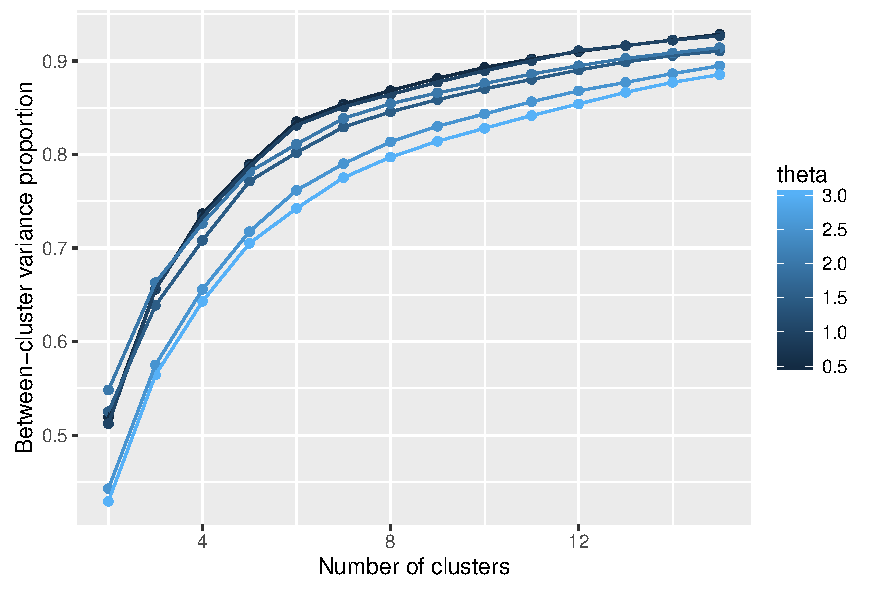
\includegraphics[width=0.49\linewidth]{Figures/CausalityRegimes/ccoef-knum_valuesFALSE_theta05-3.pdf}
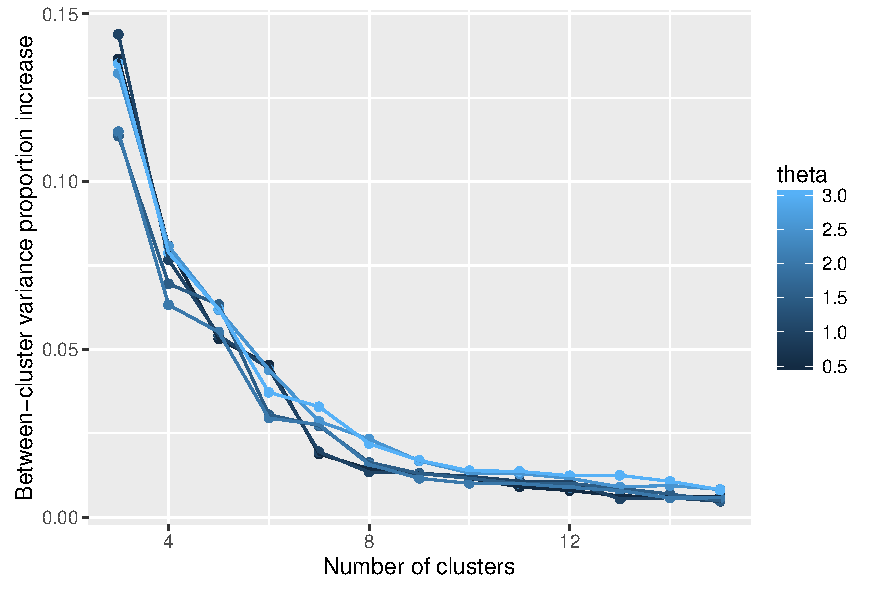
\includegraphics[width=0.49\linewidth]{Figures/CausalityRegimes/dccoef-knum_valuesFALSEtheta05-3.pdf}\\
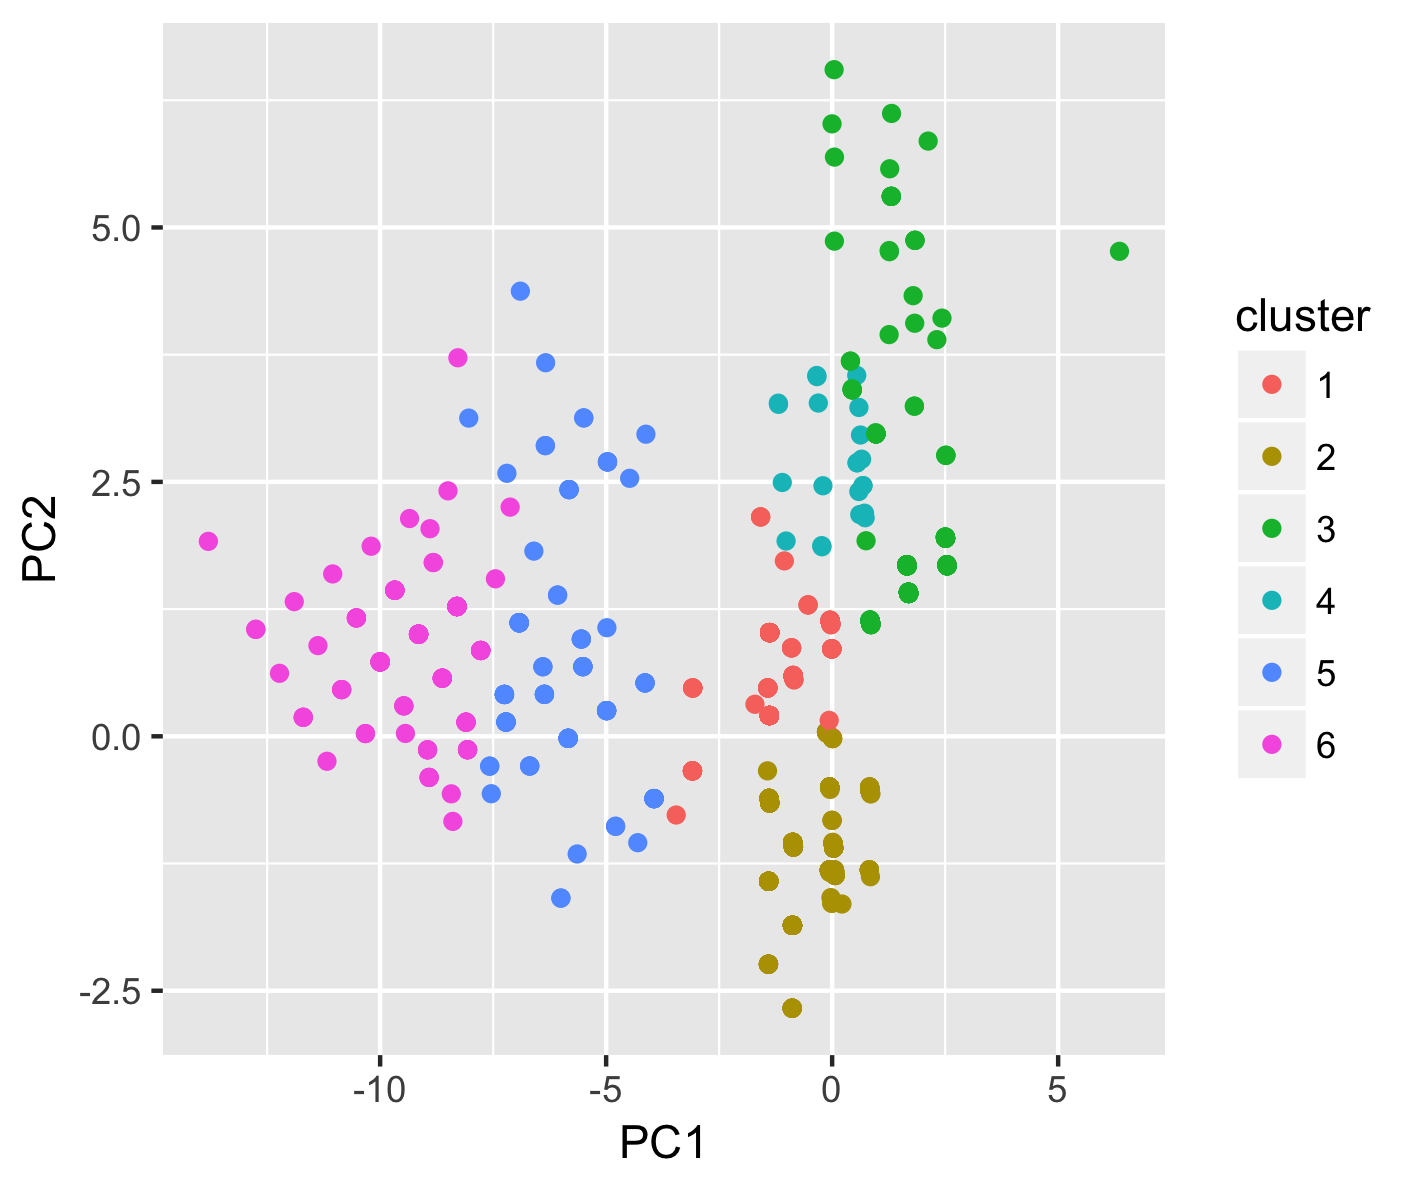
\includegraphics[width=0.4\linewidth]{Figures/CausalityRegimes/clusters-PCA-features_valuesFALSEtheta2_k6}
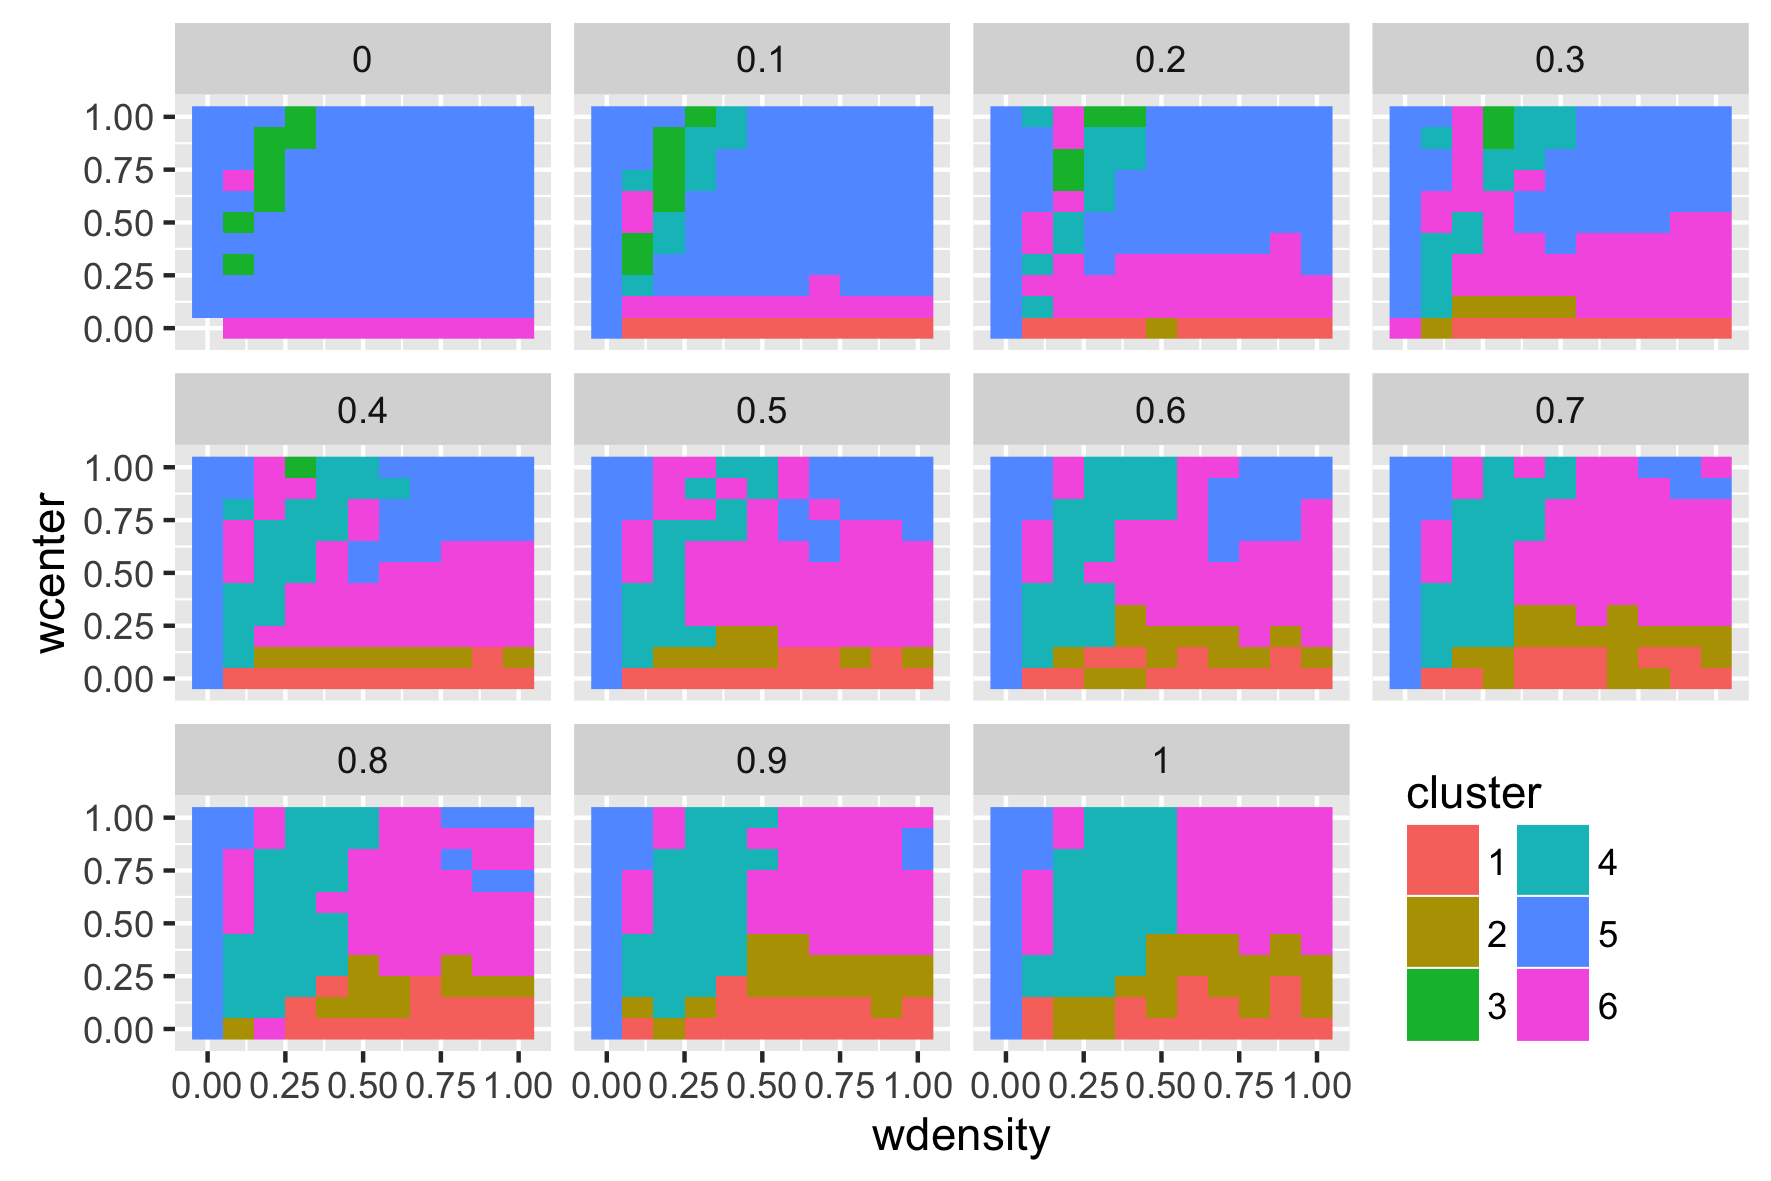
\includegraphics[width=0.59\linewidth]{Figures/CausalityRegimes/clusters-paramfacet_valuesFALSEtheta2_k6}\\
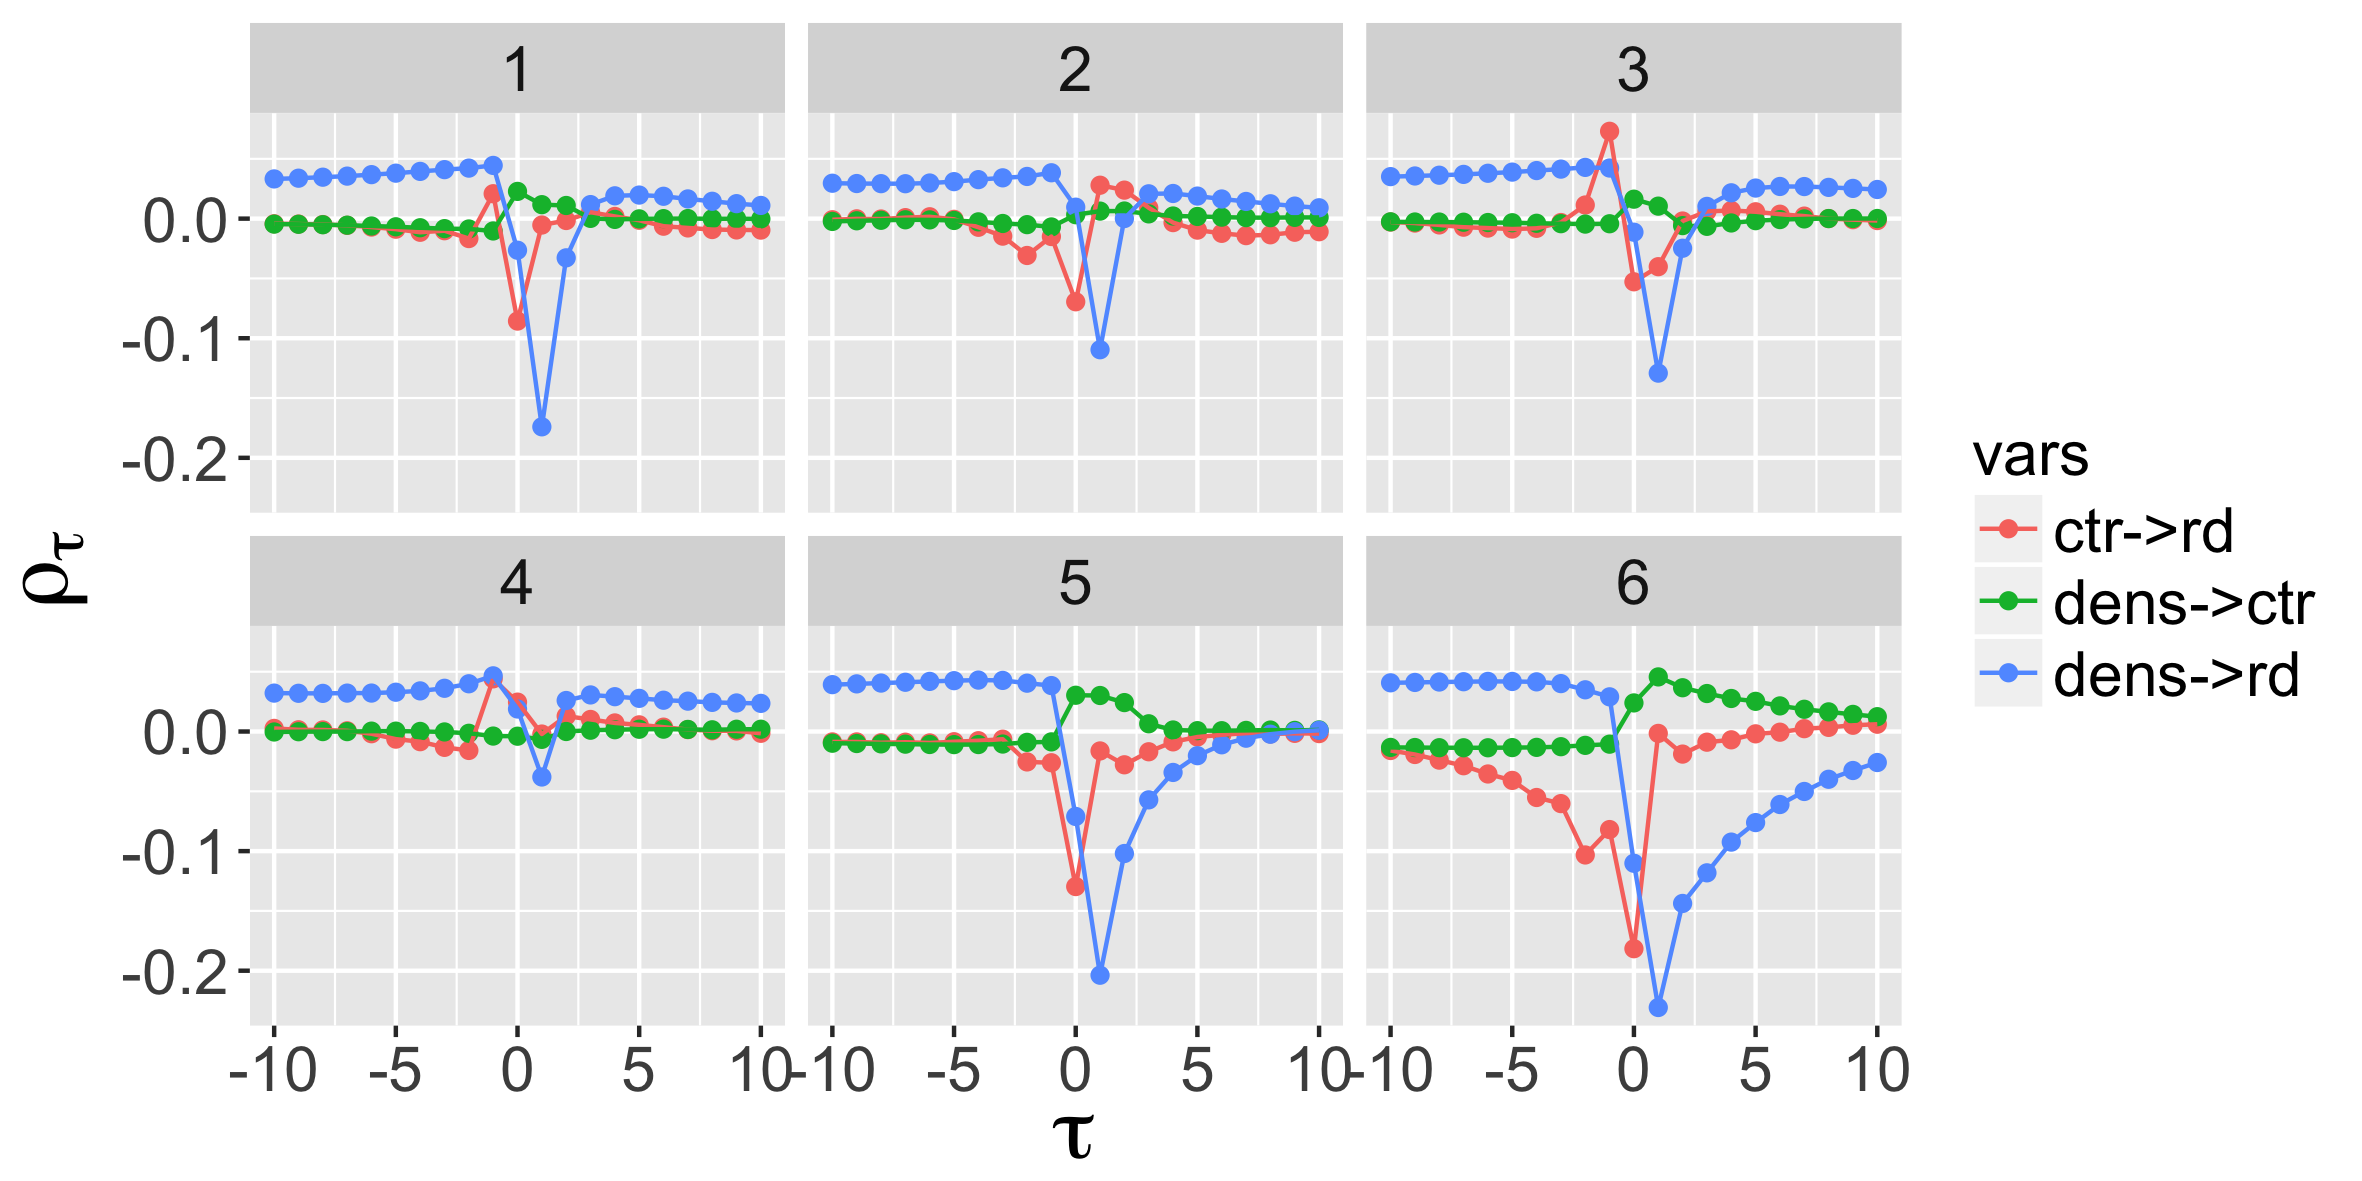
\includegraphics[width=\linewidth]{Figures/CausalityRegimes/clusters-centertrajs-facetclust_valuesFALSEtheta2_k6}
\caption[Identification of interaction regimes][Identification de régimes d'interactions]{\textbf{Identification of regimes of interaction.} \textbf{(Top left)} Inter-cluster variance as a function of cluster number. \textbf{(Top middle)} Derivative of the inter-cluster variance. \textbf{(Top right)} Features in a principal plan (81\% of variance explained by the two first components)\textbf{(Bottom left)} Phase diagram of regimes in the space $(w_{d},w_{c},w_{r})$, $w_r$ varying between the different sub-diagrams of $(w_{d},w_{c}$. \textbf{(Bottom right)} Corresponding profiles of centroids.\label{fig:causalityregimes:clustering}}{\textbf{Identification de régimes d'interactions} \textbf{(Haut Gauche)} Variance inter-cluster comme fonction du nombre de clusters. \textbf{(Haut Droite)} Dérivée de la variance inter-cluster. \textbf{(Milieu Gauche)} \emph{Features} dans un plan principal (81\% de variance expliquée par les deux premières composantes) \textbf{(Milieu Droite)} Diagramme de phase des régimes dans l'espace $(w_{d},w_{c},w_{r})$, $w_r$ variant entre les différents sous-diagrammes de $(w_{d},w_{c}$. \textbf{(Bas)} Trajectoires correspondantes des centroïdes.\label{fig:causalityregimes:clustering}}
\end{figure}
%%%%%%%%%%%%%%%



\bpar{
This method must first be tested and partially validated, what we propose to do on synthetic data, what allows a more refined knowledge of the behavior of models~\cite{raimbaulthalshs01514415}. Echoing the example of relations between transportation networks and territories that introduced the research question before, we generate stylized urban configurations in which network and density mutually interact, and for which causalities are not obvious \emph{a priori} knowing the parameters of the generative model. \cite{raimbault2014hybrid} describes and explores a simple model of urban morphogenesis (the RBD model) that fits perfectly these constraints. Indeed, explicative variables of urban growth, processes of network extension and the coupling between urban density and the network are relatively simple. However, except for extreme cases (for example when distance to the center solely determines land value, the network will depend on density in a causal way; when only the distance to the network counts, the causality will be inverted), mixed regimes do not exhibit obvious causalities. It is for this reason an ideal case to test if the method is able to detect some. We use an applied implementation\footnote{available on the open repository of the project at \\\texttt{https://github.com/JusteRaimbault/CityNetwork/tree/master/Models/Simple/ModelCA}} of the original model, allowing to capture the values of studied variables for each cell of the cellular automaton and for each time step, and to calculate the lagged correlations in the sense described before, between variables of the model. We explore a grid of the parameter space of the RBD model, making the weight parameters for density, distance to center and distance toi network vary\footnote{The model works the following way: a value of cells is determined by the weighted average of these different explicative variables, value that determines the growth of new patches at the next time step.}, that we write respectively $(w_{d},w_{c},w_{r})$, in $\left[0;1\right]$ with a step of $0.1$. Other parameters are fixed to their default values given by~\cite{raimbault2014hybrid}. For each parameter value, we proceed to $N=100$ repetitions, what is enough for a good convergence of indicators. Explorations are done with the OpenMole software~\cite{reuillon2013openmole}, the large number of simulations (1,330,000) implying the use of a computation grid. We compute for all patches the lagged correlations with the unbiased Pearson estimator between the variations of the following variables\footnote{Computing the correlations directly on the variables makes no sense since their value has no absolute meaning.}: local density, distance to center and distance to network. The figure~\ref{fig:exrdb}  shows the behavior of $\rho_{\tau}$ for each couple of variable (undirected, $\tau$ taking negative and positive values), for the combination of extreme values of parameters. We can already see different regimes emerge: for example, $(1,0,1)$ leads to a causality of density on distance to center with a lag $\tau=1$, and a negative causality of density on distance to network with the same lag, whereas distance to the center and to the network are correlated in a synchronous manner. To study these behaviors in a systematic way, we propose to identify regimes endogenously, by using non-supervised classification. We apply a \emph{k-means} clustering, robust to stochasticity (5000 repetitions), with the following features: for each couple of variables, $\textrm{argmax}_{\tau} \rho_{\tau}$ and $\textrm{argmin}_{\tau} \rho_{\tau}$ if the corresponding value is such that $\frac{\rho_{\tau}-\bar{\rho}_{\tau}}{\left|\bar{\rho}_{\tau}\right|} > \theta$ with $\theta$ threshold parameter, 0 otherwise. The inclusion of supplementary features of values of $\rho_{\tau}$ does not significantly changes the results, these are therefore not taken into account to reduce the dimension. The choice of the number of clusters $k$ is generally a difficult problem in this kind of approach~\cite{hamerly2003learning}. In our case the system exhibit an convenient structure: the curves of inter-cluster variance proportion and its derivative in figure~\ref{fig:clustering}, as a function of $k$ for different values of $\theta$, show a transition for $\theta = 2$, what gives for the corresponding curve a break around $k=6$. A visual screening of clusters in a principal plan confirms the good quality of the classification for these values. A class corresponds then to a \emph{causality regime}, for which we can represent the phase diagram as a function of model parameters, and also cluster centers profiles (computed as the barycenter in the full initial space) in figure~\ref{fig:clustering}. The behavior obtained is interesting, as regions in the diagram corresponding to the different regimes are clearly delimited and connected. For example, we observe the emergence of regime 6 in which distance to network causes strongly the density in a negative way, but distance to the center causes distance to the network. Its maximal extent on $(w_d,w_r)$ is for an intermediate value $w_r=0.7$. Thus, to maximize the impact of network on density, the corresponding weight must not be maximized, what can be counter-intuitive at first sight. It illustrates the utility of the method in the case of circular causal relations difficult to entangle a priori. The regime 5, in which distance to network influences the density the same way, but the relation between distance to center and to the network is inverted, is also interesting, and predominates for low $w_r$ values. The regime 1 is an extreme one and corresponds to an isolated situation in which distance to the center has no role: this aspect dominates then totally the other interaction processes between density and network. This application on synthetic data demonstrate on one hand the robustness of the method given the consistence of obtained regimes, and realizes this way a much more finer qualification of model behavior than the one done in the original paper. In this precise case, it can be taken as an instrument of knowledge for relations between networks and territories in itself, allowing the test of assumption or the comparison of processes in the stylized model.
}{
Cette méthode doit dans un premier temps être testée et partiellement validée, ce que nous proposons de faire sur des données synthétiques, méthode qui permet une connaissance plus fine des comportements des modèles~\cite{raimbault2016generation}. En écho à l'exemple des relations entre réseaux de transport et territoires qui a permis d'introduire notre problématique précédemment, nous proposons de générer des configurations urbaines stylisées dans lesquelles réseau et densité s'influencent mutuellement, et pour lesquelles les causalités ne sont pas évidents \emph{a priori} étant donné les paramètres du modèle génératif. \cite{raimbault2014hybrid} décrit et explore un modèle simple de morphogenèse urbaine (modèle RBD) répondant parfaitement à ces contraintes. En effet, les variables explicatives de la croissance urbaine, les processus d'extension du réseau et le couplage entre densité urbaine et réseau ne sont pas trop complexes. Cependant, hormis dans des cas extrêmes (par exemple lorsque la distance au centre détermine la valeur foncière uniquement, le réseau dépendra de manière causale de la densité, ou lorsque la distance au réseau seule compte, la causalité sera inversée), les régimes mixtes n'exhibent pas de causalités évidentes : c'est donc un parfait cas pour tester si la méthode est capable d'en détecter. Nous utilisons une implémentation adaptée\footnote{disponible sur le dépôt ouvert du projet à\\\texttt{https://github.com/JusteRaimbault/CityNetwork/tree/master/Models/Simple/ModelCA}} du modèle initial, permettant de capturer les valeurs des variables étudiées pour chaque patch et à chaque pas de temps et de calculer les correlations retardées entre variables au sein du modèle. Nous explorons une grille de l'espace des paramètres du modèle RBD, faisant varier les paramètres de poids de la densité, de la distance au centre et de la distance au réseau\footnote{Le modèle fonctionne de la façon suivante : une valeur des patches est déterminée par la moyenne pondérée de ces différentes variables explicatives, valeur qui détermine la croissance de nouveaux patches à l'instant suivant.}, que l'on note respectivement $(w_{d},w_{c},w_{r})$, dans $\left[0;1\right]$ avec un pas de 0.1. Les autres paramètres sont fixés à leur valeurs par défaut données par \cite{raimbault2014hybrid}. Pour chaque valeur des paramètres, nous procédons à $N=100$ répétitions ce qui est suffisant pour une bonne convergence des indicateurs. Les explorations sont effectuées via le logiciel OpenMole~\cite{reuillon2013openmole}, le grand nombre de simulations (1,330,000) nécessitant l'utilisation d'une grille de calcul. Nous calculons sur l'ensemble des patches les corrélations retardées par estimateur de Pearson non biaisé entre les variations des variables suivantes\footnote{Calculer les corrélations sur les variables directement n'a pas de sens puisque leur valeur n'en a pas en absolu.} : densité locale, distance au centre et distance au réseau. La Fig.~\ref{fig:causalityregimes:exrdb} montre le comportement de $\rho_{\tau}$ pour chaque couple de variable (non dirigé, $\tau$ prenant des valeurs négatives et positives), pour les combinaisons des valeurs extrêmes des paramètres. On peut voir déjà différents régimes émerger : par exemple, $(1,0,1)$ conduit à une causalité de la densité sur la distance au centre avec un retard 1, et une causalité négative de la densité sur la distance au réseau avec le même retard, tandis que distance au centre et au réseau sont corrélés de manière synchrone. Afin d'étudier ces comportements de manière systématique, nous proposons d'identifier des régimes de manière endogène, en procédant à un apprentissage non-supervisé. Nous appliquons une classification des \emph{k-means}, robuste à la stochasticité (5000 répétitions), avec les points caractéristiques (\emph{features}) suivants : pour chaque couple de variable, $\textrm{argmax}_{\tau} \rho_{\tau}$ et $\textrm{argmin}_{\tau} \rho_{\tau}$ si la valeur correspondante est telle que $\frac{\rho_{\tau}-\bar{\rho}_{\tau}}{\left|\bar{\rho}_{\tau}\right|} > \theta$ avec $\theta$ paramètre de seuil, 0 sinon. L'inclusion des \emph{features} supplémentaires des valeurs de $\rho_{\tau}$ n'influence pas significativement les résultats, celles-ci n'ont pas été prises en compte pour réduire la dimension. Le choix du nombre de clusters $k$ est en général épineux dans ce genre de problème~\cite{hamerly2003learning}, dans notre cas le système possède une structure agréable : les courbes de la proportion de variance inter-cluster et de sa dérivée en Fig.~\ref{fig:causalityregimes:clustering}, en fonction de $k$ pour différentes valeurs de $\theta$, présentent une transition pour $\theta = 2$, ce qui donne pour cette courbe une rupture à $k=5$. Un examen visuel des clusters dans un plan principal confirme la bonne qualité de la classification pour ces valeurs. Une classe correspond alors à un \emph{régime de causalité}, dont nous pouvons représenter le diagramme de phase en fonction des paramètres du modèle, ainsi que les trajectoires des centres des clusters (calculées comme barycentre dans l'espace complet initial) en Fig.~\ref{fig:clustering}. Le comportement obtenu est particulièrement intéressant : les régions du diagramme correspondant aux régimes sont clairement délimitées et connexes. Par exemple, on observe l'émergence du régime 6 où la distance au réseau cause fortement la densité de manière négative, mais la distance au centre cause la distance au réseau, régime dont l'étendu maximale sur $(w_d,w_r)$ est pour une valeur intermédiaire $w_r=0.7$. Ainsi, pour maximiser l'impact du réseau sur la densité, il ne faut pas maximiser le poids correspondant, ce qui peut paraître contre-intuitif en premier abord : cela illustre l'intérêt de la méthode dans le cas de relations circulaires difficiles à démêler a priori. Le régime 5, où la distance au réseau influence la densité de la même manière, mais la relation entre distance au centre et route est inversée, est tout aussi intéressant, et est prédominant dans les faibles $w_r$. Le régime 1, extrême, correspond à une situation isolée dans laquelle la distance au centre n'importe pas : cet aspect domine alors totalement les autres processus d'interaction entre densité et réseau. Cette application sur données synthétique démontre ainsi d'une part la robustesse de la méthode vu la cohérence des régimes obtenus, et constitue aussi une qualification beaucoup plus précise des comportements du modèle que celle réalisée dans l'article initial. Dans ce cas précis, il peut s'agir d'un instrument de connaissance des relations entre réseaux et territoires en lui-même, permettant le test d'hypothèses ou la comparaison de processus dans le modèle stylisé.
\comment[FL]{ces explications sont difficiles a lire car ce n'est pas assez hierarchise}
}


















%--------------------------------------------------------









%%%%%%%%%%%%%%%%%%%%%%%
\subsection{Network-territory relations in South Africa}{Relations Réseaux-territoires en Afrique du Sud}



\bpar{
We assum that territorial dynamics and network dynamics responded differently to these. We expect to learn from these project informations on interactions at long time scale and large spatial scale, in a very particular context of constrained growth.
}{
Nous démontrons à présent les potentialités de notre méthode sur des données géo-historiques sur le temps long, pour le cas du réseau ferré en Afrique du Sud au cours du 20ème siècle. En faisant l'hypothèse que les territoires et les réseaux réagissent différemment aux événements historiques, les motifs de causalité devraient informer sur leur relations sur le temps long.
}


\subsubsection{Context}{Contexte}


\bpar{
Transportation Networks can be leveraged as a powerful socio-economic control tool, with even more significant outcomes when it percolates to their interaction with territories. The case of South Africa is an accurate illustration, as \cite{baffi:tel-01389347} shows that during apartheid railway network planning was used as a racial segregation tool by shaping strongly constrained mobility and accessibility patterns. In particular, it is shown qualitatively that dynamics between territories and networks profoundly changed at the end of the apartheid, transforming a tool of planed segregation (network shaped was optimized to minimize unwanted accessibility) into an integration tool thanks to recent changes in network topology patterns. We propose to investigate the potential \emph{structural} properties of this historical process, by focusing on dynamical patterns of interactions between the railway network and city growth. More precisely, we try to establish if the segregative planning policies did actually modify the trajectory of the coupled system, what would correspond to deeper and wider impacts. 
}{
Les réseaux de transport peuvent être utilisés comme un puissant outil de contrôle socio-économique, avec des effets encore plus significatifs lorsque ceux-ci perturbent les relations avec les territoires. Le cas de l'Afrique du Sud est une illustration pertinente, puisque \noun{Baffi} montre dans~\cite{baffi:tel-01389347} que lors de l'apartheid la planification du réseau ferré était utilisée comme un outil de ségrégation raciale par l'établissements de motifs de mobilité et d'accessibilité fortement contraints. En particulier, il est montré qualitativement que les dynamiques entre réseaux et territoires ont profondément changé à la fin de l'apartheid, transformant un outil de ségrégation planifiée (une forme de réseau optimisée pour minimisée une accessibilité non désirée) en un outil d'intégration grâce à des changement récents dans la topologie du réseau. Nous étudions ici les potentielles propriétés \emph{structurelles} de ce processus historique, en se concentrant sur les motifs dynamiques des interactions entre le réseau ferré et la croissance des villes. Plus précisément, nous essayons d'établir si les politiques de planification ségrégatives ont effectivement modifié la trajectoire du système couplé, ce qui correspondrait à des impacts plus larges et profonds que leurs effets immédiats.
}





\subsubsection{Results}{Résultats}


\paragraph{Data}{Données}


\bpar{
We use a comprehensive database covering the full South African railway network from 1880 to 2000 with opening and closing dates for each station and link, together with a city database spanning from 1911 to 1991 for which consistent ontologies for urban areas have been ensured. These database are described by~\cite{baffi:tel-01389347}, but they are not open so we make available only the aggregated data we used in the analysis.
}{
Nous utilisons une base de données complète couvrant l'ensemble du réseau ferré Sud-Africain de 1880 à 2000 avec les dates d'ouverture et de fermeture pour chaque station et liaison, couplée à une base de données pour les villes s'étendant de 1911 à 1991 pour laquelle des ontologies consistantes pour les aires urbaines ont été assurées. Ces bases de données sont décrites par~\cite{baffi:tel-01389347}, mais ne sont pas ouvertes, nous mettons ainsi à disposition uniquement les données agrégées utilisées dans l'analyse.\comment[FL]{a mettre dans une partie type ch3, ulterieurement}
}



\paragraph{Network Measures}{Mesures de réseau}

\bpar{
First, a dynamical study of network measures seem to confirm the hypothesis: a trend rupture in closeness centrality (defined for a node as the average travel time to other nodes) at a roughly constant network size evolution, at a date corresponding to the beginning of official segregative policies, suggests that the planning process after this date had in the best case no global effect on network performance, and in the worst case had intended negative effects on accessibility with the aim to physically segregate more.
}{
Une analyse préliminaire consiste à regarder l'évolution dynamique des mesures de réseau, celles-ci pouvant témoigner de ruptures dans les propriétés structurelles du réseau et donc de mutations historiques profondes. L'évolution de certaines propriétés du réseau, comme les distributions de la centralité ou de l'accessibilité, peut témoigner l'existence d'une planification les ayant influencées. Nous montrons en Figure~\ref{fig:causalityregimes:network} l'évolution des mesures de réseau dans le temps, correspondant aux mesures les plus basiques de celles définies en~\ref{sec:staticcorrelations}. La centralité de proximité, que nous définissons comme le temps moyen de trajet vers les autres noeuds, présente un comportement intéressant. En effet, la taille du réseau et les valeurs moyennes des centralités présentent un comportement concordant, qui correspond à l'expansion initiale du réseau. Par contre, la tendance de la hiérarchie de la centralité de proximité à se réduire est soudainement rompue à la date correspondant à l'officialisation des politiques ségrégatives en 1951, alors que taille et forme géométrique globale du réseau, traduite par l'efficience, restent constants. Ainsi, la planification après cette date a dans le meilleur des cas eu aucun effet sur cette propriété, dans le pire des cas est en effet responsable de cette rupture de tendance, c'est à dire a eu les effets escomptés sur l'accessibilité, dans le but d'empêcher la diminution de la ségrégation, puisque plus la hiérarchie est faible plus le réseau est égalitaire.
}


%%%%%%%%%%%%%%
\begin{figure}[h!]
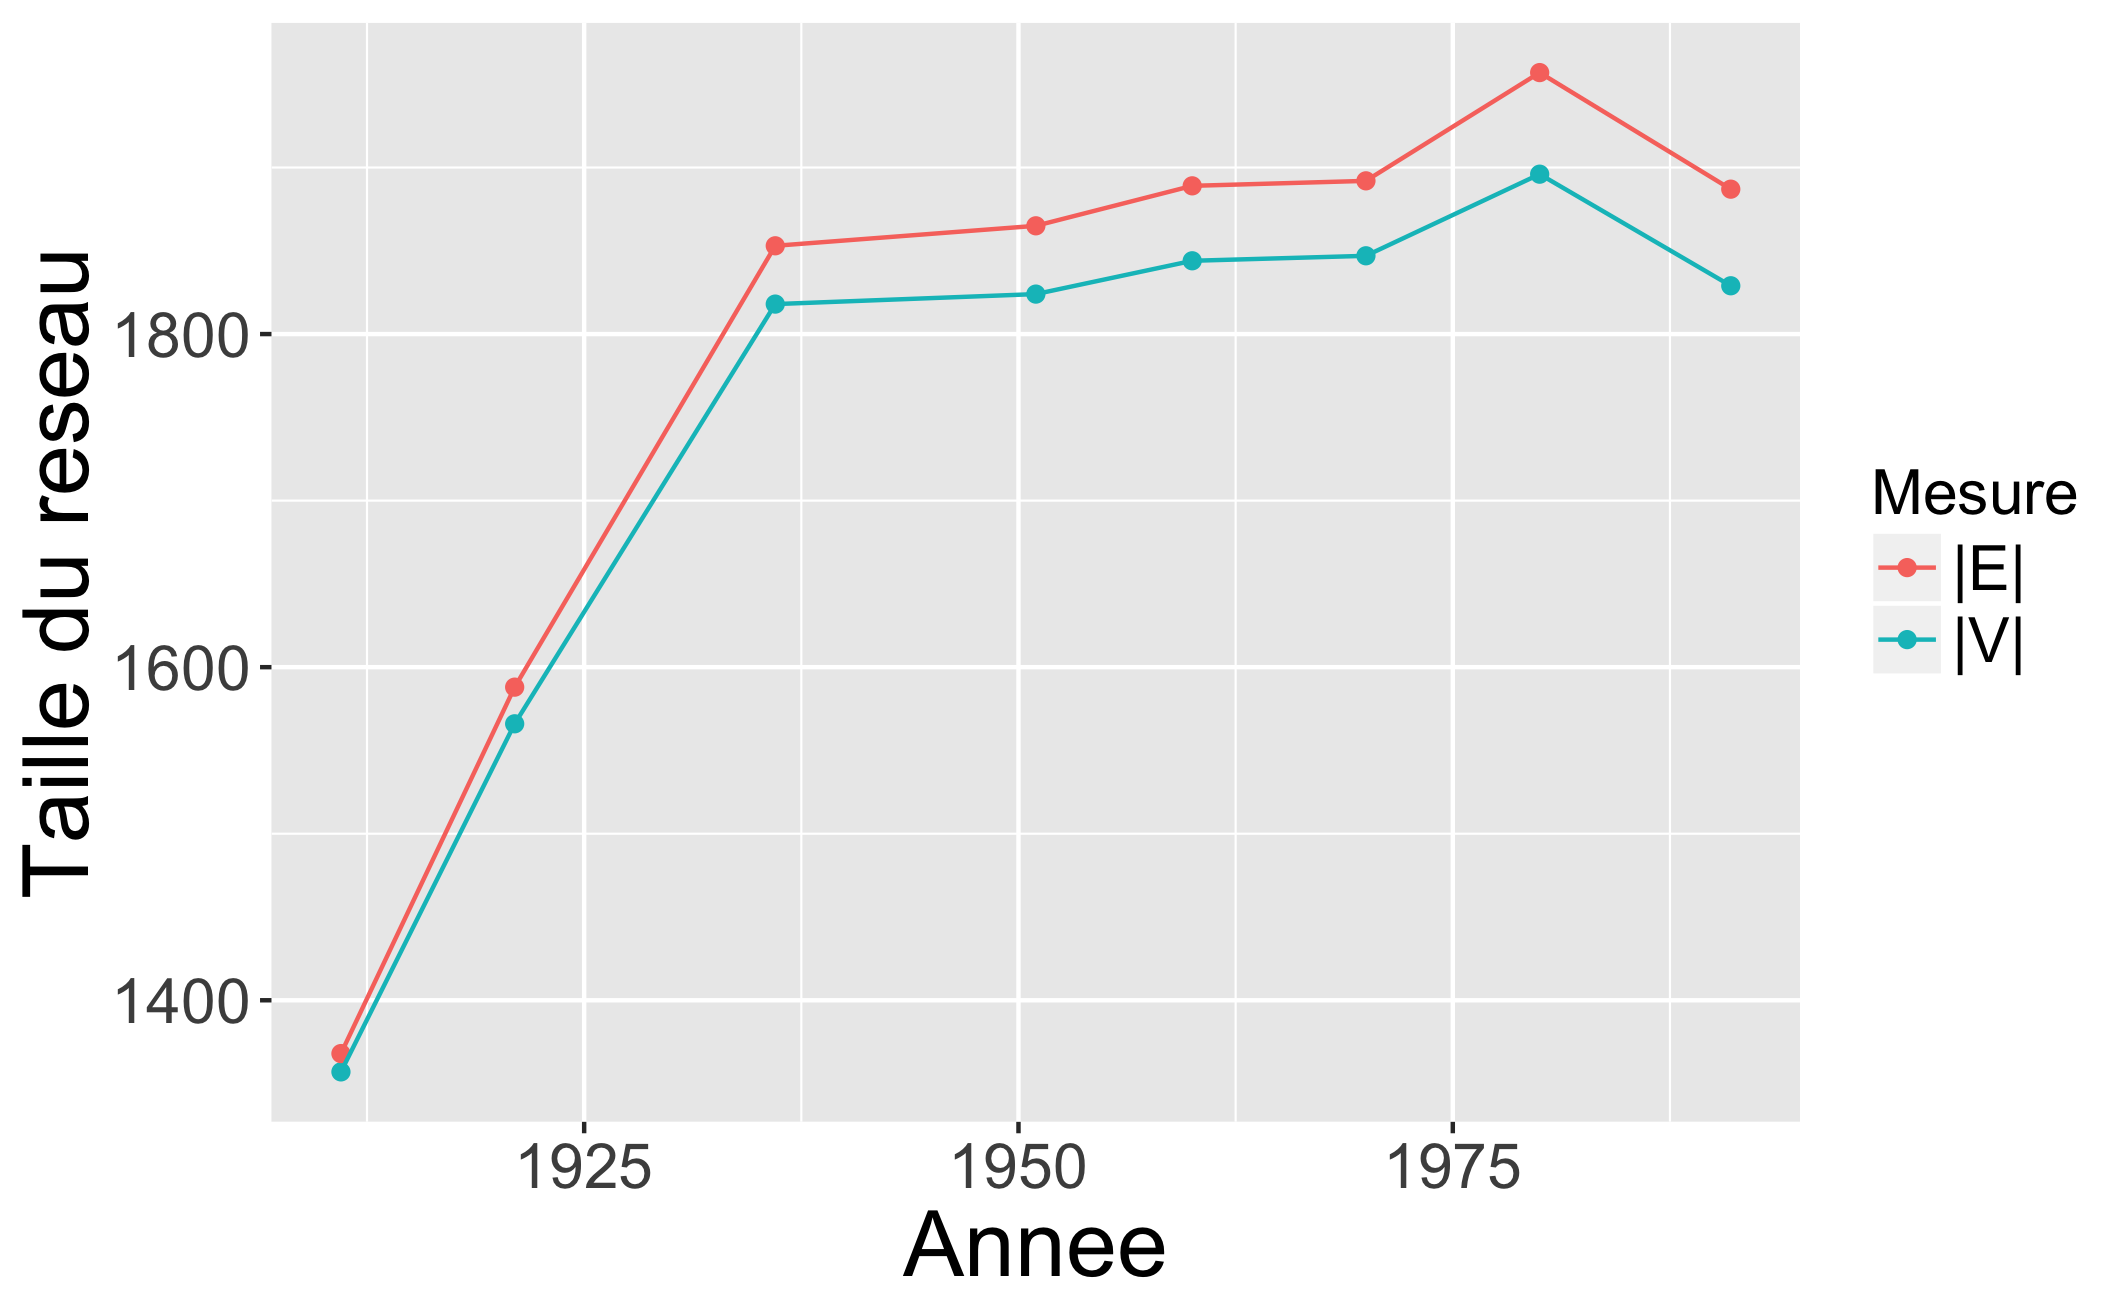
\includegraphics[width=0.42\linewidth]{Figures/CausalityRegimes/nw_nwSize}
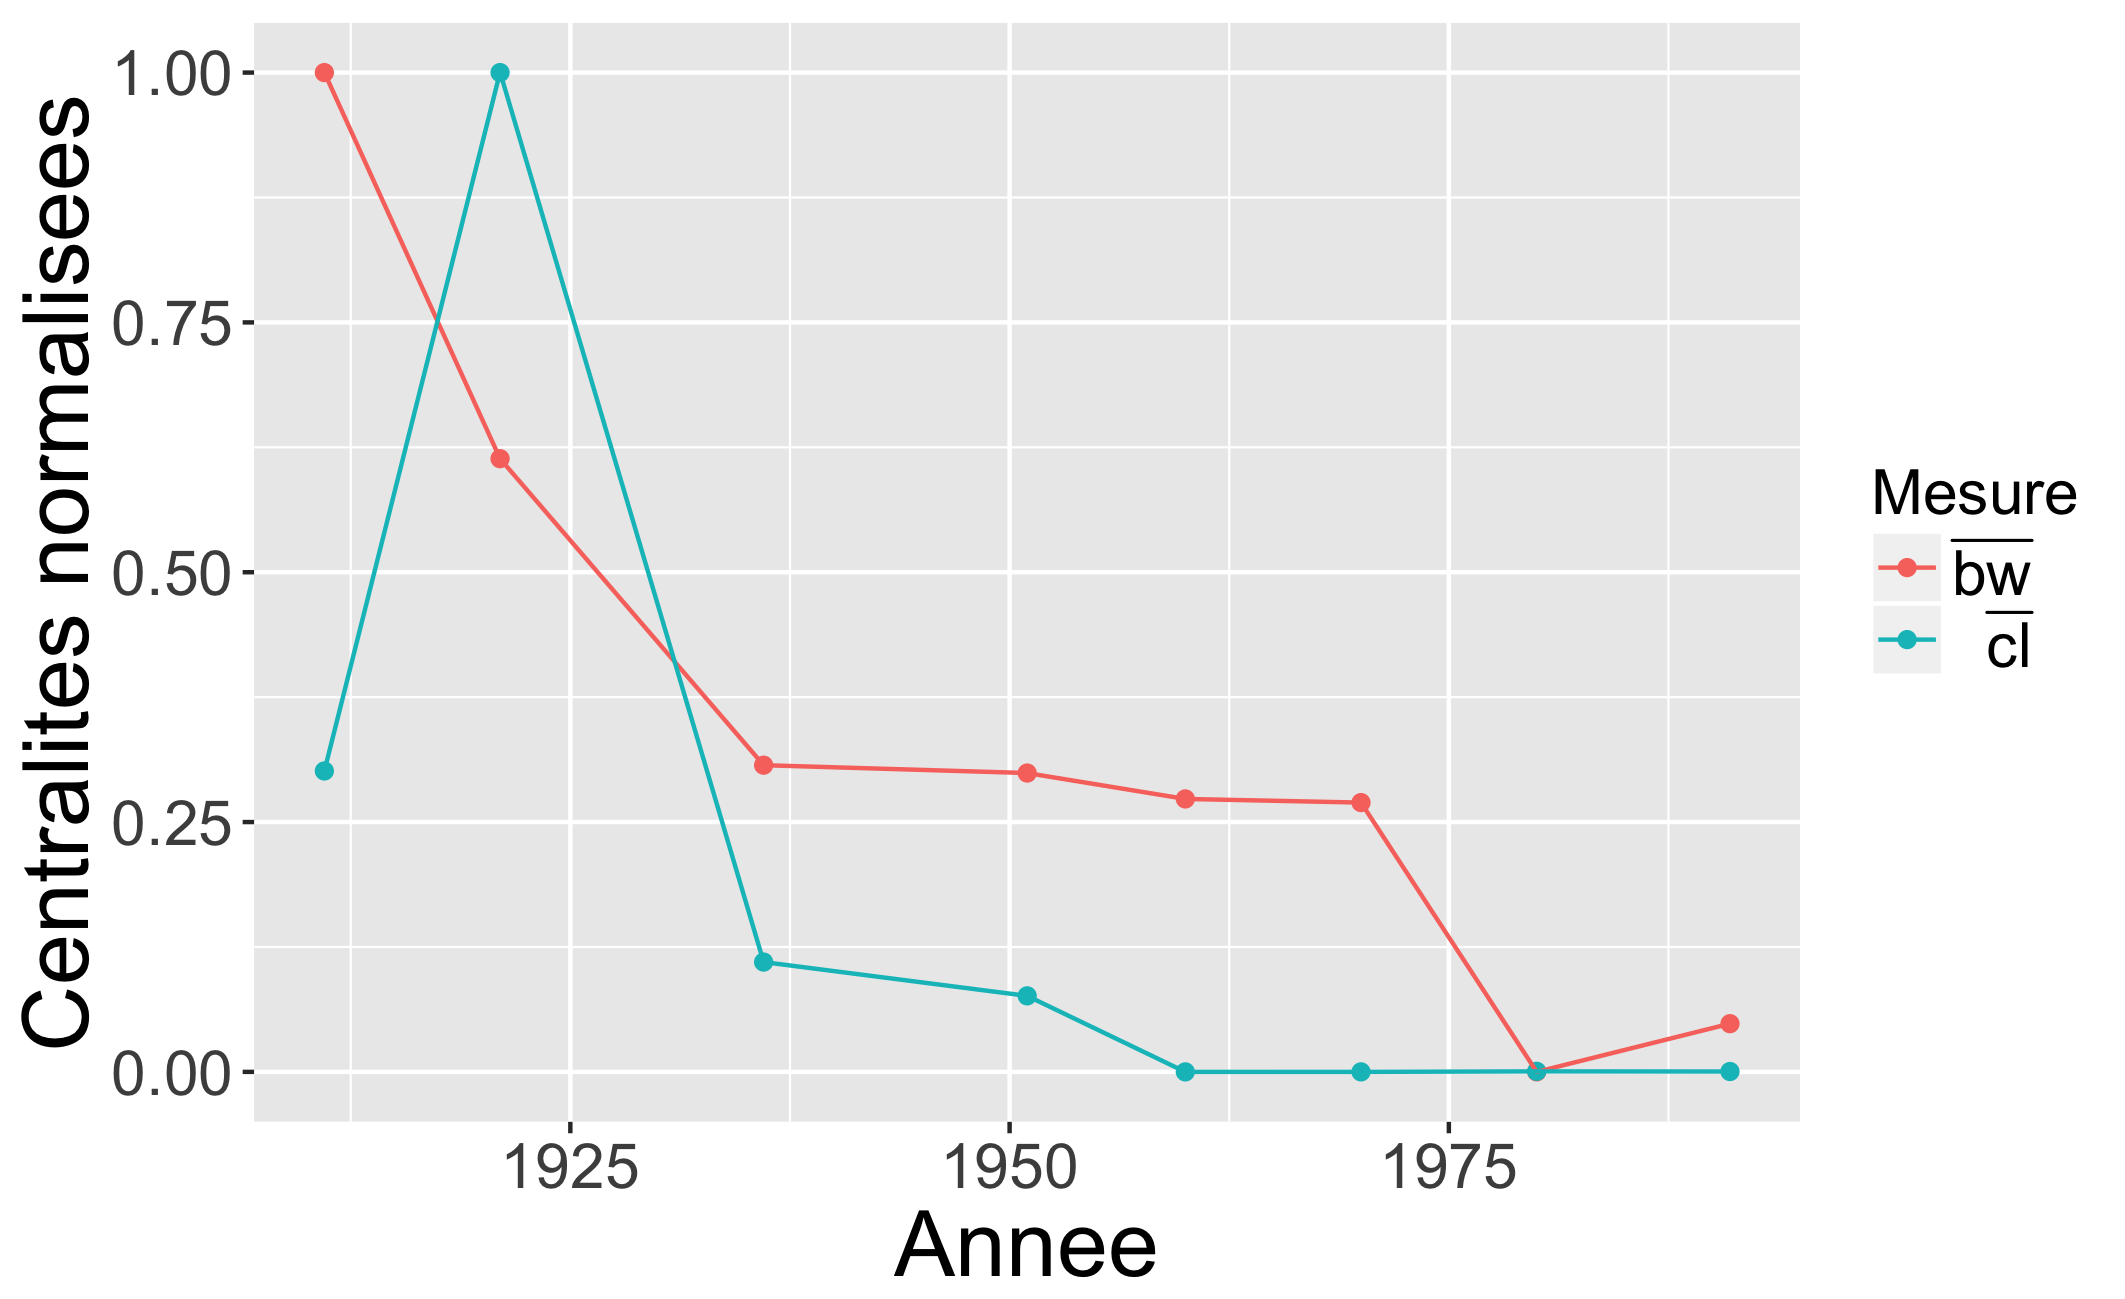
\includegraphics[width=0.47\linewidth]{Figures/CausalityRegimes/nw_meanCentralities}\\
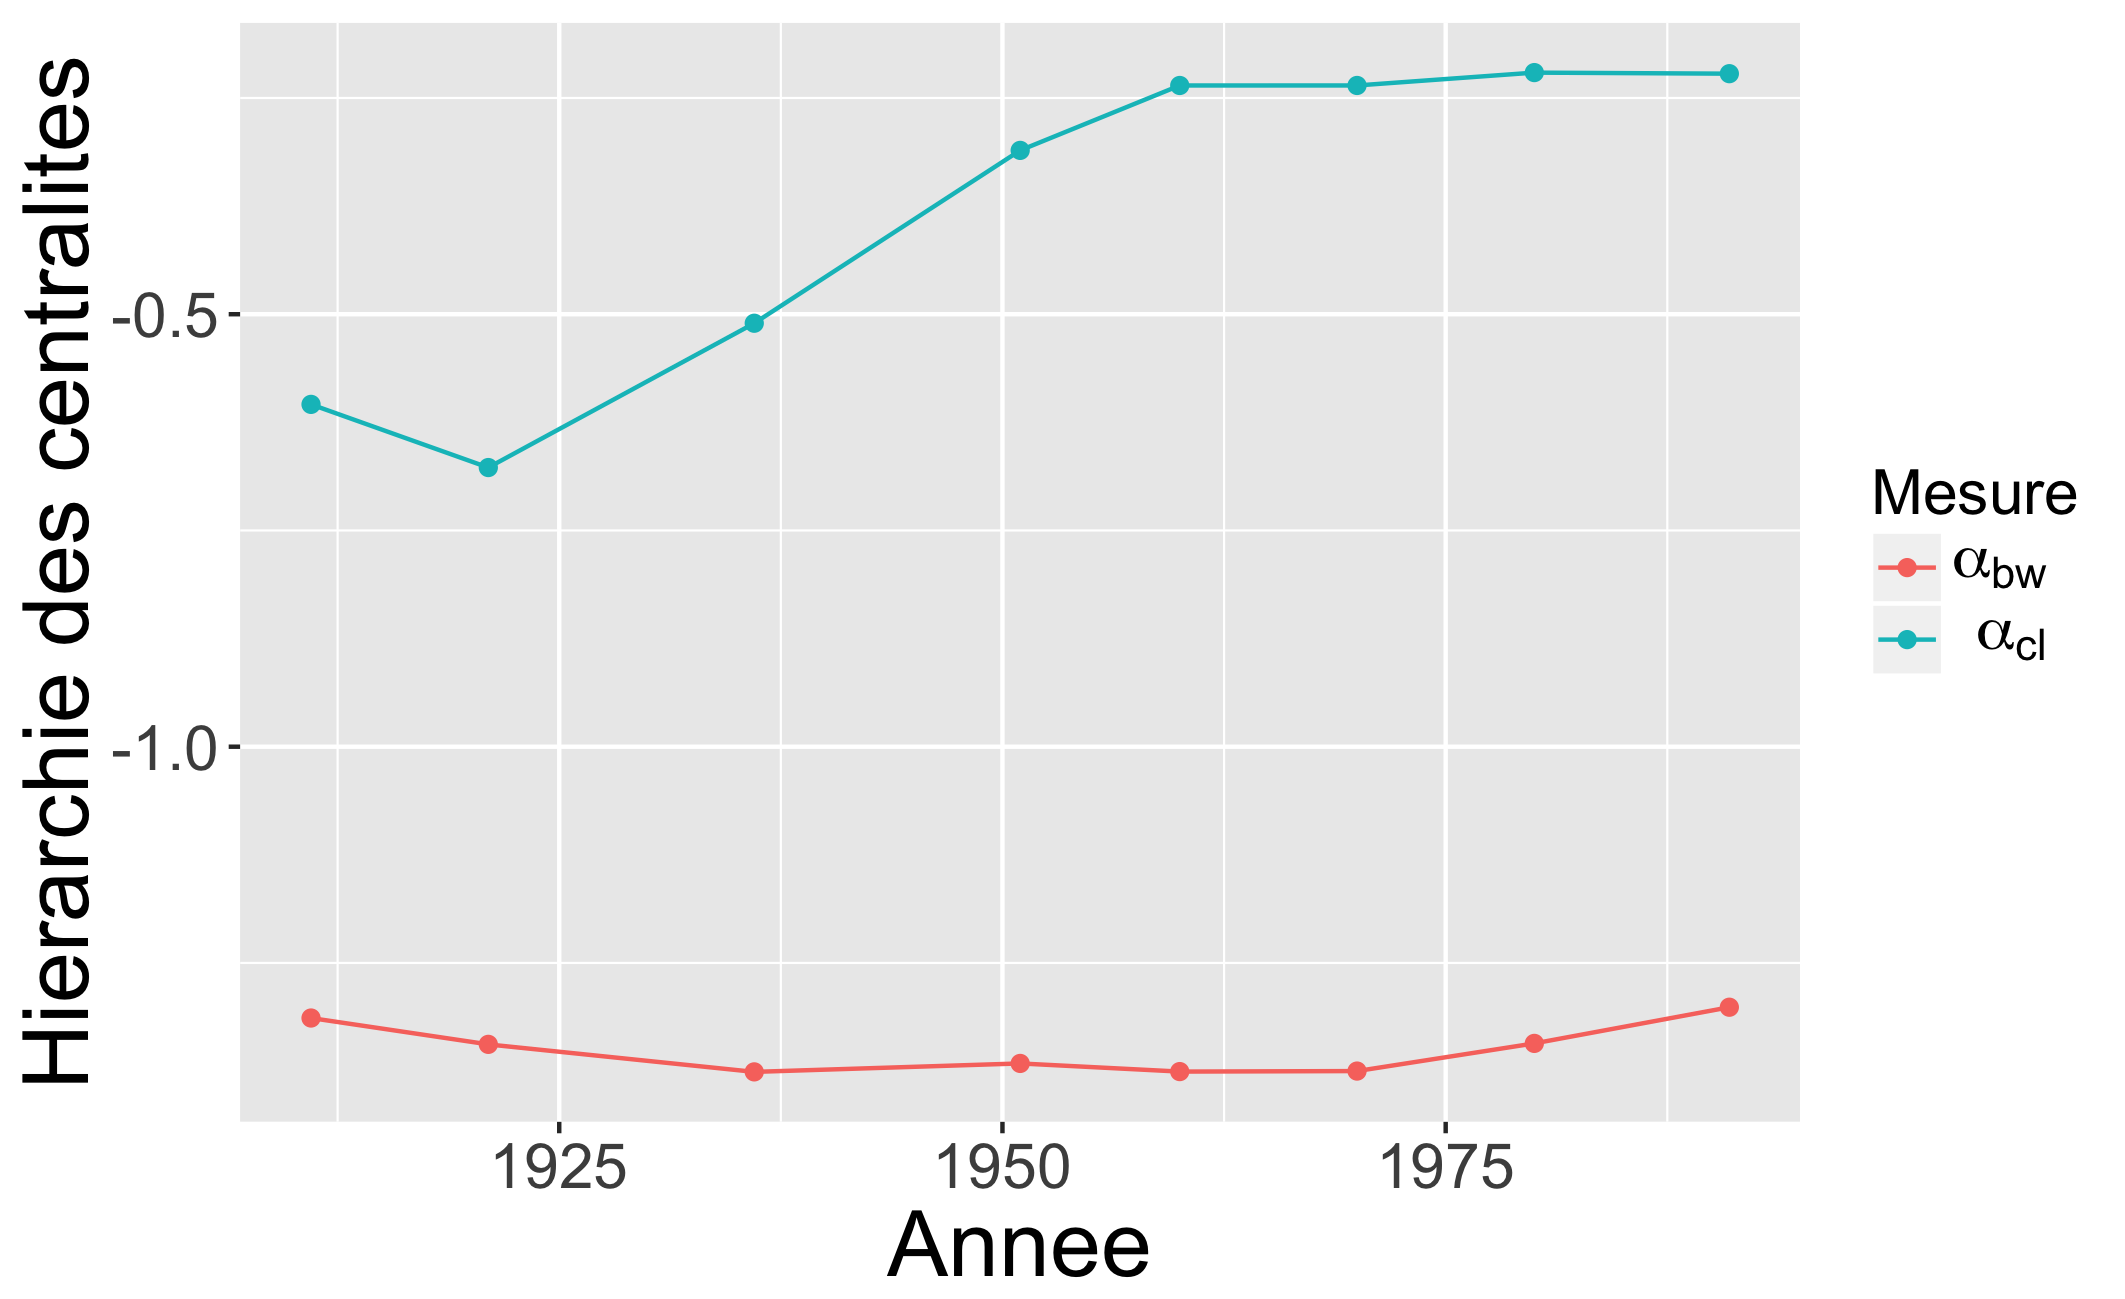
\includegraphics[width=0.48\linewidth]{Figures/CausalityRegimes/nw_hierarchies}
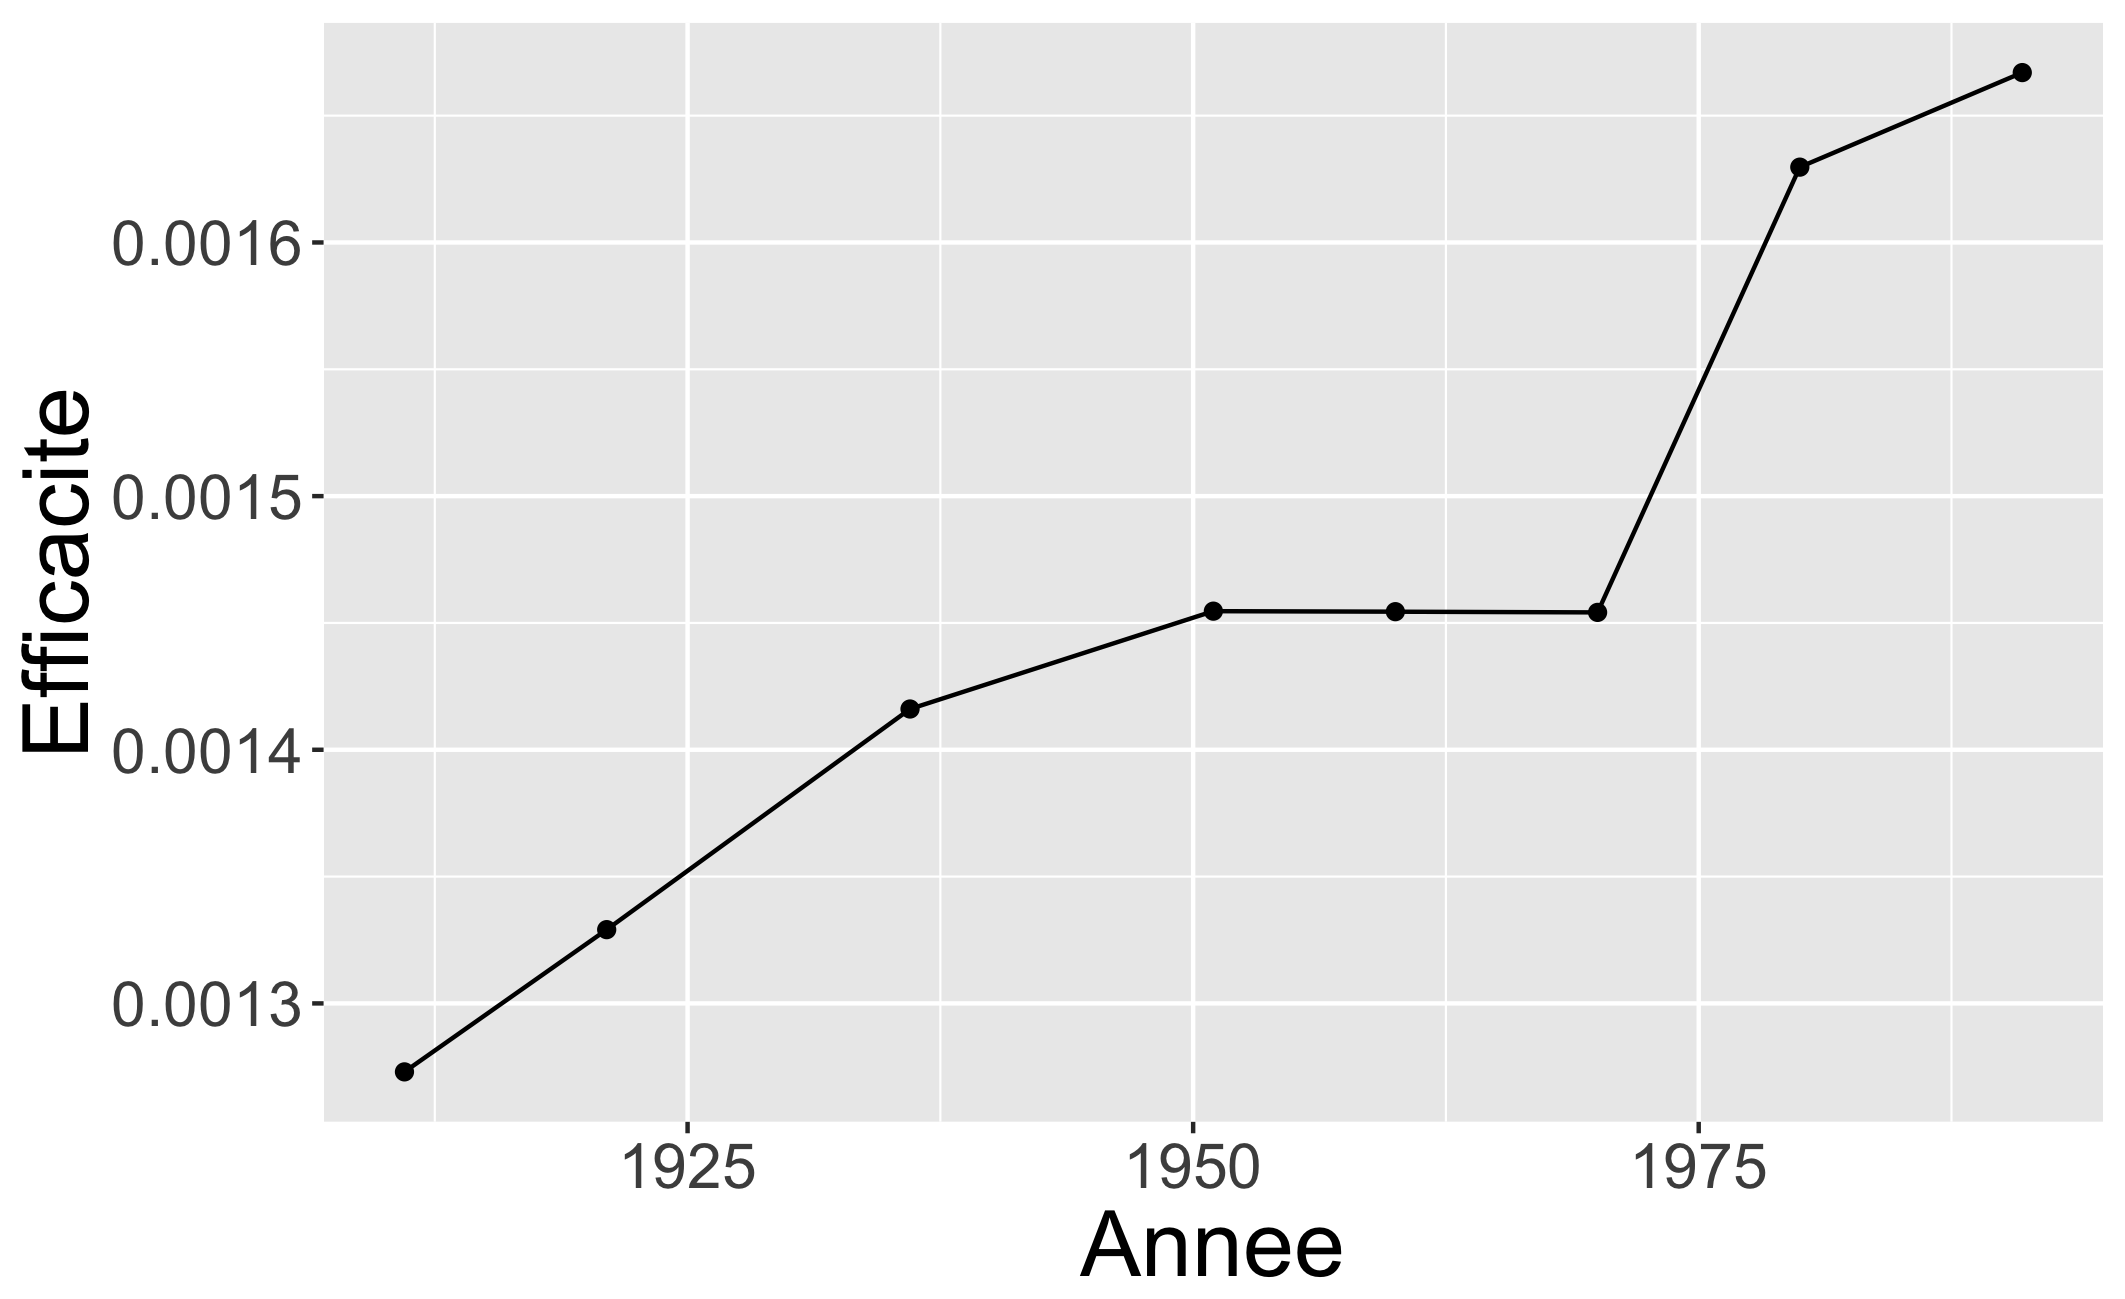
\includegraphics[width=0.41\linewidth]{Figures/CausalityRegimes/nw_efficiency}
\caption[Evolution of network measures][Evolution des mesures de réseau]{\label{fig:causalityregimes:network}}{\textbf{Evolution des mesures de réseau.} On calcule pour l'ensemble des dates les mesures basiques de réseau : taille, centralités résumées par leur hiérarchie et leur moyenne, efficience. Les centralités sont normalisées pour comparaison de leur variation respective ($\max \bar{bw} = 0.07$, $\max \bar{cl} = 1.5e-4$).\label{fig:causalityregimes:network}}
\end{figure}
%%%%%%%%%%%%%%



\paragraph{Causality patterns}{Motifs de causalité}


\bpar{
We then turn to dynamical interactions between the railway network and city growth. For that, we study Granger causalities, in the large sense of correlations between lagged variables, estimated between cities growth rates and accessibility differentials due to network growth, for all cities and urban areas having a connection to the network.
We test both travel-time and population weighted accessibilities, for varying values of distance decay parameter. Lagged correlations are fitted on varying length time windows, to test for potentially varying stationarity scales. Results are shown in Figure~\ref{fig:causalityregimes:sudafcorrs}. We find that results are significant with travel-time accessibility only, autocorrelation dominating with weighted accessibility. A time-window of 30 years appears to be a good compromise between the number of significant correlations ($p<0.1$ for a Fisher test) and the absolute correlation level across all lags and distance decays, what should correspond roughly to the time-stationarity scale of the system. We observe furthermore a phase transition when distance decay increases, revealing the shift between the spatial scale of urban areas and the scale of the country, what gives local spatial stationarity scale. We obtain therethrough clear causality patterns, namely an inversion of the Granger causality (lagged correlation up to 0.5 for several values of distance decay), from accessibility causing population growth with a lag of 10-20 years before the apartheid (1948), to the opposite after the apartheid (lag 20 years). We interpret these as \emph{Structural segregation}, i.e. a significant impact of planning policies on dynamics of interactions between networks and territories. Indeed, the first regime corresponds to direct effect of transportation on migrations in a free context in opposition to the second one.
}{
Nous examinons à présent les interactions dynamiques entre le réseau ferré et la croissance urbaine. Pour cela, nous appliquons la méthode développée dans la première partie, qui consiste à l'étude des causalités de Granger, au sens large des corrélations entre les variables retardées, estimées entre les taux de croissance des villes et les différentiels d'accessibilité dus à la croissance du réseau, pour toutes les villes ou aires urbaines ayant une connection au réseau. Nous testons à la fois l'accessibilité en terme de distance et pondérée par la population à l'origine et aux deux extrémités. Si $P_i$ sont les populations, $d_{ij}$ la matrice de distance dans le réseau, l'accessibilité de $i$ sera donnée par $Z_i = w_i \sum_j w_j \exp \left(- d_{ij} / d_0 \right)$ où $d_0$ est le paramètre de décroissance et les poids $w_i$ sont $1/N$ ou $P_i / \sum_j P_j$ selon la modalité. Nous faisons varier les valeurs de $d_0$ pour prendre en compte les relations à différentes échelles spatiales. De plus les corrélations retardées sont estimées sur des fenêtres temporelles de taille variable $T_W$, pour tester différentes échelles de stationnarité temporelles potentielles. Les résultats des estimations sont montrés en Figure~\ref{fig:causalityregimes:sudafcorrs}. Nous obtenons des résultats significatifs avec l'accessibilité non-pondérée seulement, l'auto-corrélation devant dominer l'accessibilité pondérée : en effet, on a pour les deux variables pondérées des valeurs positives pour les faibles valeurs de $d_0$ uniquement, les autres n'étant pas significatives. Le meilleur compromis pour la fenêtre temporelle apparaît être une trentaine d'année, si on cherche à avoir à la fois un bon nombre de corrélations significatives (définies par $p<0.1$ pour un test de Fisher) et le niveau moyen de corrélation absolue sur l'ensemble des retards et des paramètres de décroissance. Nous interprétons cette valeur comme approximativement l'échelle de stationnarité du système. De plus, le nombre de corrélations significatives exhibe clairement une transition de phase dans ses valeurs intermédiaires, ce qui devrait correspondre au passage entre l'échelle spatiale des aires urbaines et celle du pays, ce qui donne l'échelle locale de stationnarité spatiale. Quand on examine le comportement des corrélations retardées pour la distance, on observe des motifs de causalité assez évident, puisque le sens de la causalité de Granger s'inverse autour de 1950, celle-ci étant à chaque fois marquée par des corrélations allant jusqu'à 0.5 pour certaines valeurs du paramètre de décroissance. On passe ainsi d'une accessibilité causant la croissance de la population avec un délai de 10 à 20 ans avant l'apartheid (1948), à l'opposé après l'apartheid (avec un délai de 20 ans). Nous interprétons ce phénomène comme une \emph{ségrégation structurelle}, c'est à dire un impact significatif des politiques de planification sur les dynamiques des interactions entre les réseaux et les territoires. En effet, on peut interpréter le premier régime comme un effet direct du transport sur les motifs de migration dans un contexte de liberté, en opposition au second régime qui correspondrait à un contrôle de la population et d'une adaptation du réseau en fonction. Ainsi, l'évènement historique a eu un effet au second ordre sur les relations dynamiques.
}


%%%%%%%%%%%%%%
\begin{figure}[h!]
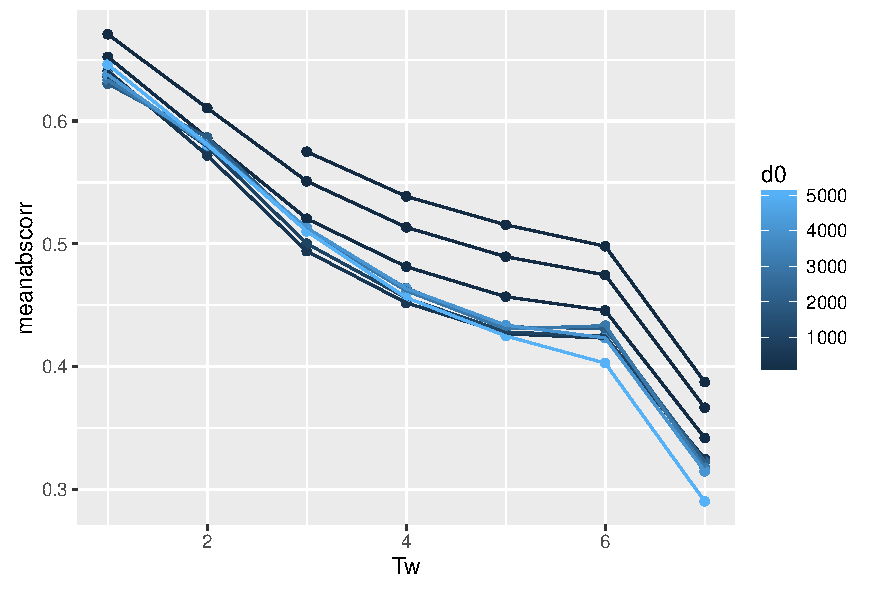
\includegraphics[width=0.49\linewidth]{Figures/CausalityRegimes/meanabscorrs}
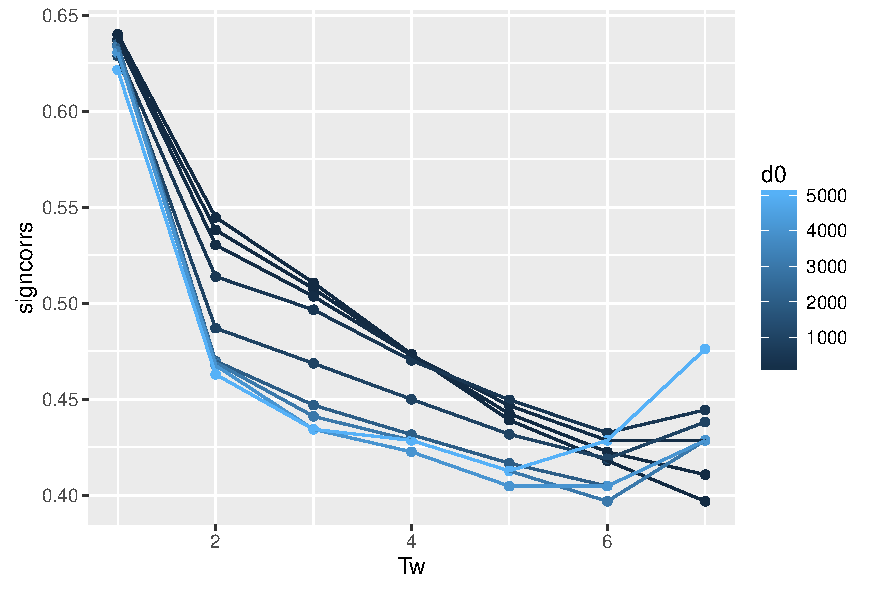
\includegraphics[width=0.49\linewidth]{Figures/CausalityRegimes/significantcorrs}\\
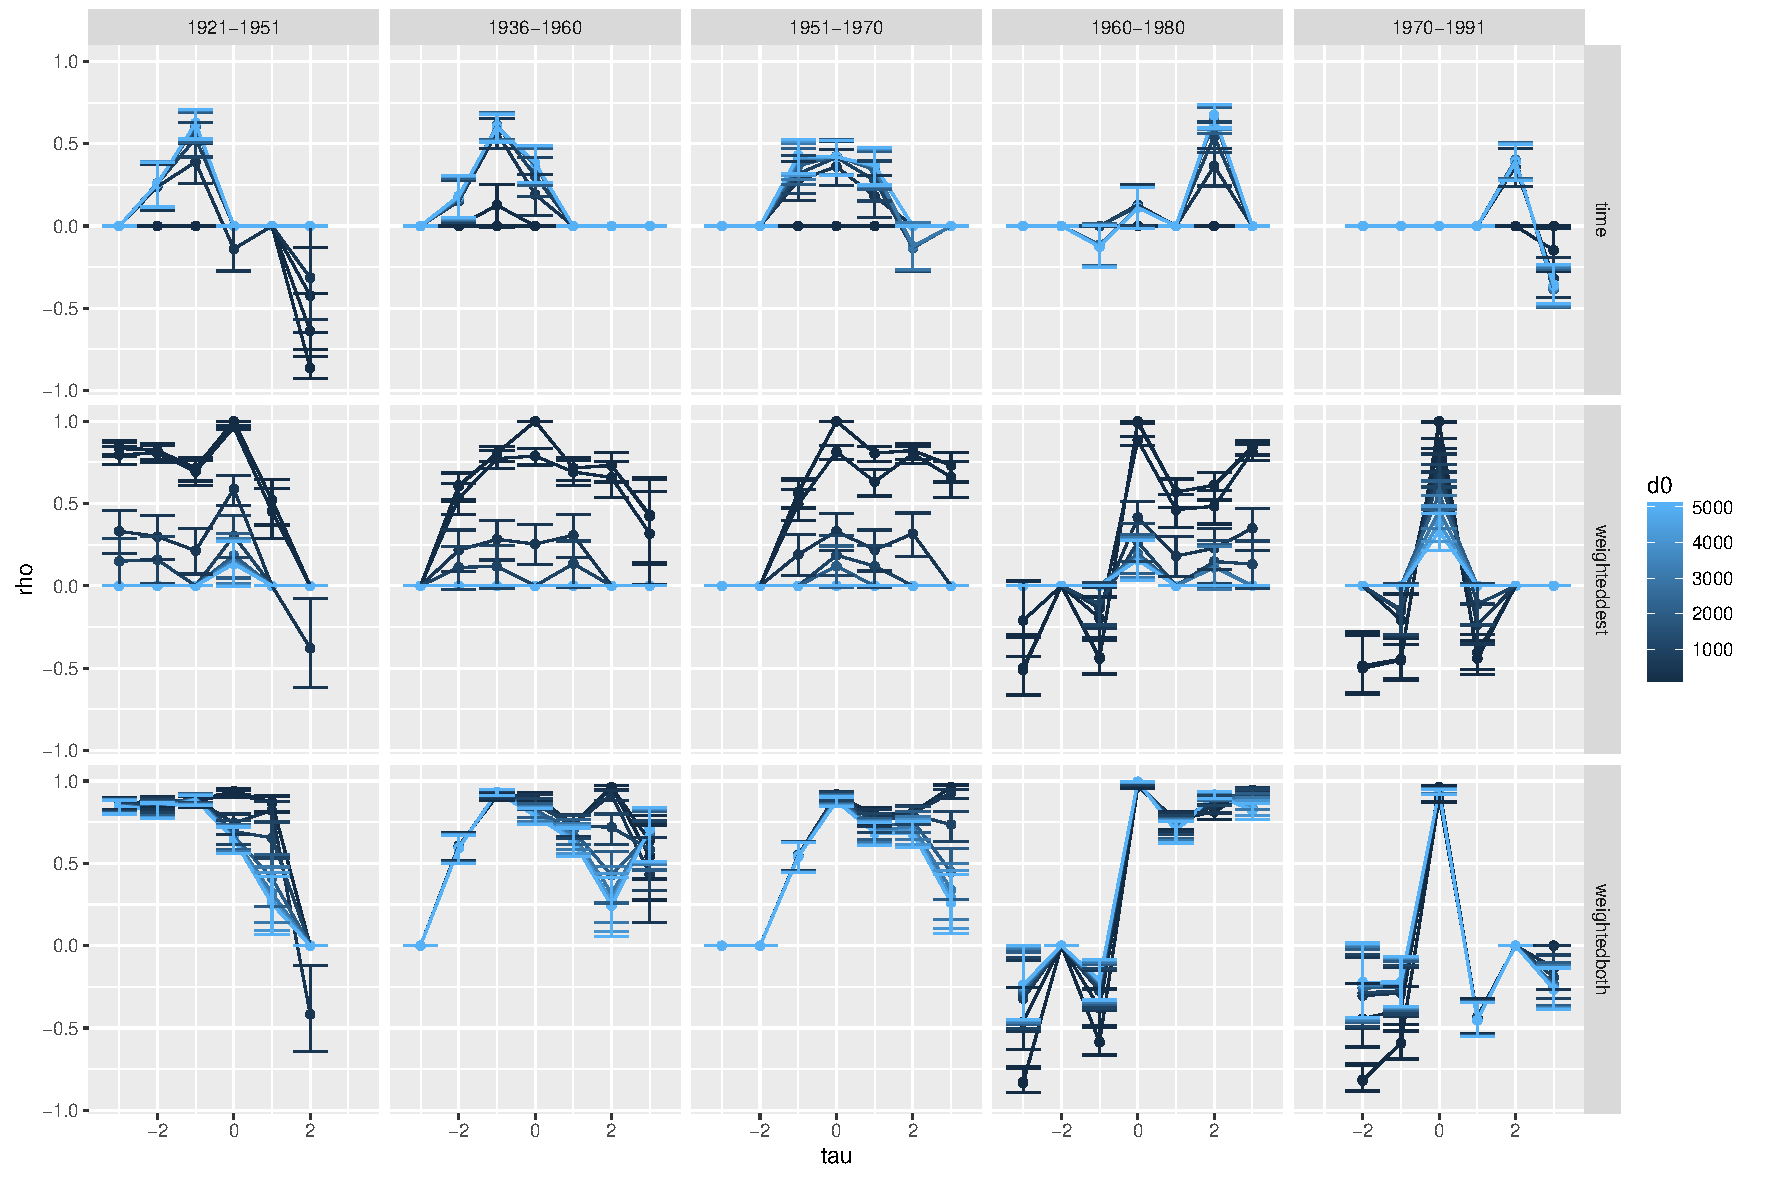
\includegraphics[width=\linewidth]{Figures/CausalityRegimes/laggedCorrs_Tw3}
\caption[Lagged correlations][Corrélations retardées]{\label{fig:causalityregimes:sudafcorrs}}{\textbf{Corrélations retardées.} \textit{(Haut Gauche)} Corrélations absolues moyennées sur l'ensemble des retards, en fonction de la taille de la fenêtre temporelle $T_W$ (en nombre d'observations temporelles), pour différentes valeurs du paramètre de décroissance $d_0$ ; \textit{(Haut Droite)} Proportion de corrélations significatives, en fonction de $T_W$ pour $d_0$ variable ; \textit{(Bas)} Corrélations retardées en fonction du délai $\tau$, pour la taille optimale $T_W=3$, sur les différentes périodes successives (colonnes), pour les différents degrés de pondérations (première ligne $w_i=1$, deuxième ligne $w_i = 1,w_j=P_j/\sum_k P_k$, troisième ligne $w_i = P_i/\sum_k P_k,w_j=P_j/\sum_k P_k$), et pour $d_0$ variable (couleur).\label{fig:causalityregimes:sudafcorrs}\comment[FL]{impossible a comprendre}}
\end{figure}
%%%%%%%%%%%%%%


\subsubsection{Possible developments}{Développements possibles}

\bpar{
Further work should consist in similar study with more precise socio-economic variables, for example quantifying directly segregation patterns. The method of instruments in statistics~\cite{angrist1996identification} is used to identify causal relationships between variables, in a different way than Granger causality test for example. Trying to identify causalities between network dynamics and territorial dynamics is of crucial importance to test our theoretical assumption on the existence of co-evolution.
}{
Une première extension pourra consister en une étude similaire avec des variables socio-économiques plues précise, pour quantifier par exemple directement les motifs de ségrégation. D'autre part, des variables qualitatives liées aux évènements historiques pourraient faire office de variable d'instrumentation. La méthode des variables instrumentales~\cite{angrist1996identification} est utilisée pour identifier des relations causales entre variables, d'une façon complémentaire à celle que nous avons mis en place. On pourrait chercher à rendre nos conclusions plus robustes, notamment vérifier si les corrélations ne sont pas fortuites, par l'application de cette approches. \comment[FL]{a la fin on ne sait pas ce que tu as prouve car tu ne le raccroches pas a de la literature existante}
}








\stars









